\chapter{Creating an Efficient Database Infrastructure for Discovery of Real Materials Exemplified with High Entropy Alloys} \label{chap:ultera}

\section{Introduction} \label{ultera:sec:intro}

Compared to atomic structures discussed in Chapters \ref{chap:sipfenn} through \ref{chap:crystall}, which are precisely defined, "real" materials which were physically made in a lab tends to be (a) much less homogeneous in terms of \textit{how} they are reported and (b) the data belonging to them is much less defined in terms of the \textit{completeness} of description, i.e., many critical parameters like phases present can be missing or misreported due to a plethora of reasons including lack of equipment, limited precision, or human errors. Because of these, handling them generally requires much more flexible and elaborate ecosystem capable of:
\begin{enumerate}
    \item Handling voids in the knowledge with a structured, well-defined, reproducible procedures. 
    \item Filling in the gaps using the prior knowledge and available domain coverage.
    \item Detect unavoidable errors coming from humans, machines, and miscommunications along a long path from when the data is conceived (e.g., \textit{"This alloy should be strong and ductile"}), through initial report (e.g., \textit{"Sample 17 (A17) was X [...] Tensile tests were performed. [...] A17 fractured at 0.172"}), to the database (e.g., \textit{"X has tensile ductility of 17.2\%"}).
\end{enumerate}

One of the most challenging examples of handling "real" materials are compositionally complex materials (CCMs), and their sub-class of high entropy alloys (HEAs) \cite{Yeh2004NanostructuredOutcomes, Cantor2004MicrostructuralAlloys}, also known as multi principle element alloys (MPEAs) \cite{Borg2020ExpandedAlloys} which cover a broad spectrum of chemical elements with several of them present simultaneously, making their exploration both conceptually and computationally challenging, as explored in detail in later chapters (see Section \ref{nimplex:ssec:compositionallycomplex}). Further complexity arises from relatively high experimental and computational cost of studying them, causing researchers to typically focus on 1 to 4 property measurements (2.8 on average), while leaving at least several properties of interest undefined. Thus, it becomes critical to be able to combine multiple studies into a homogeneous structure that can be used collectively in as complete as possible form.

This has been largely accomplished for HEAs within the ULTERA, or ULtrahigh TEmperature Refractory Alloys project performed under the ARPA-E ULTIMATE program \cite{ULTIMATEArpa-e.energy.gov}, described in this Chapter, that has been continuously built and expanded since 2021 \cite{Debnath2021GenerativeAlloys} alongside associated machine learning efforts \cite{Debnath2023ComparingAlloys} and experimental validations \cite{Li2024DesignExperiments}. Within ULTERA, every property data serving as the core of the database is structured into Material - Property - Reference - Metadata quadruplet, as depicted along with sub-fields in Figure~\ref{ultera:fig:material}.

\begin{figure}[H]
    \centering
    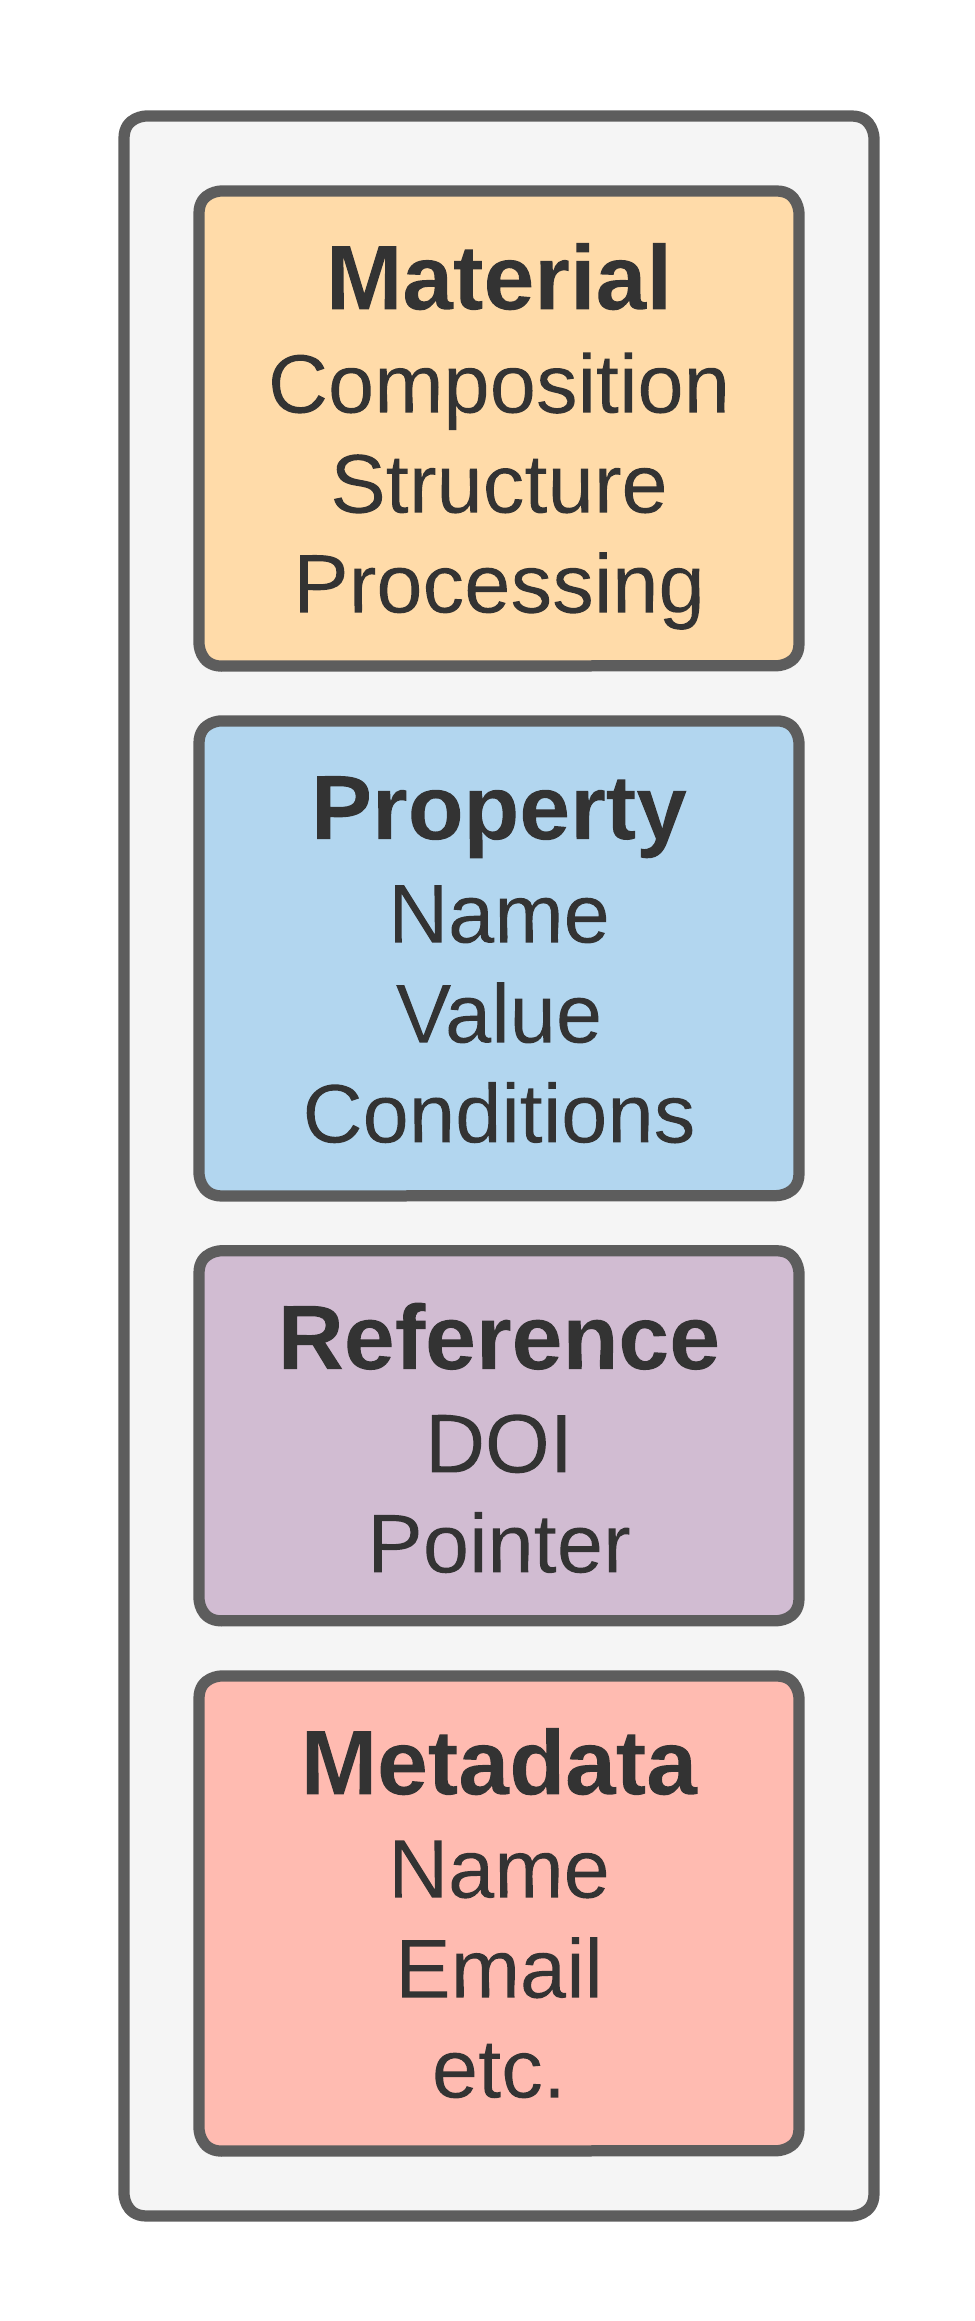
\includegraphics[width=0.2\textwidth]{ultera/ULTERA Data Detail_material.png}
    \caption{Underlying core data overview.}
    \label{ultera:fig:material}
\end{figure}

This core structure is then populated with dataset in Section~\ref{ultera:sec:datadescription} using infrastructure described in Sections~\ref{ultera:sec:infrastructure} to \ref{ultera:sec:contributions}, while being expanded and filled using several automated modeling methods described in Section \ref{ultera:sec:automodel}.


\section{Dataset} \label{ultera:sec:datadescription}
\newcommand{\statisticstime}{April 2024}

The dataset of the ULTERA Database has been manually collected through efforts of several ULTERA team members specializing in different properties, augmented with a few manually collected literature datasets processed through curation and aggregation data pipelines described in Section \ref{ultera:sec:pipeline}. All data was then further curated through \texttt{PyQAlloy} software described in Chapter \ref{chap:pyqalloy}, typically resulting in $5-10\%$ of the data points being modified to match original publications or removed.

After all the data processing steps, which generally reduced the number of datapoints and prioritized original studies over larger collections, as of \statisticstime, $\approx54\%$ of the property datapoints has been collected internally by ULTERA team, $\approx39\%$ from internally-improved version of dataset by \citet{Borg2020ExpandedAlloys}, $\approx5\%$ from \citet{Yang2022AHardness}, and $\approx3\%$ from \citet{Wang2023SearchingExperiments}. Collectively, over 550 scientific publications have been parsed to arrive at nearly 7,000 individual \textit{experimental} property datapoints, with further 500 coming from computer-based methods, belonging to nearly 3,000 unique materials spanning nearly 2,000 distinct chemical compositions, as presented in Figure~\ref{ultera:fig:dashboard}, which can be accessed in its most current form under \href{https://ultera.org}{ultera.org} project website.

\begin{figure}[H]
    \centering
    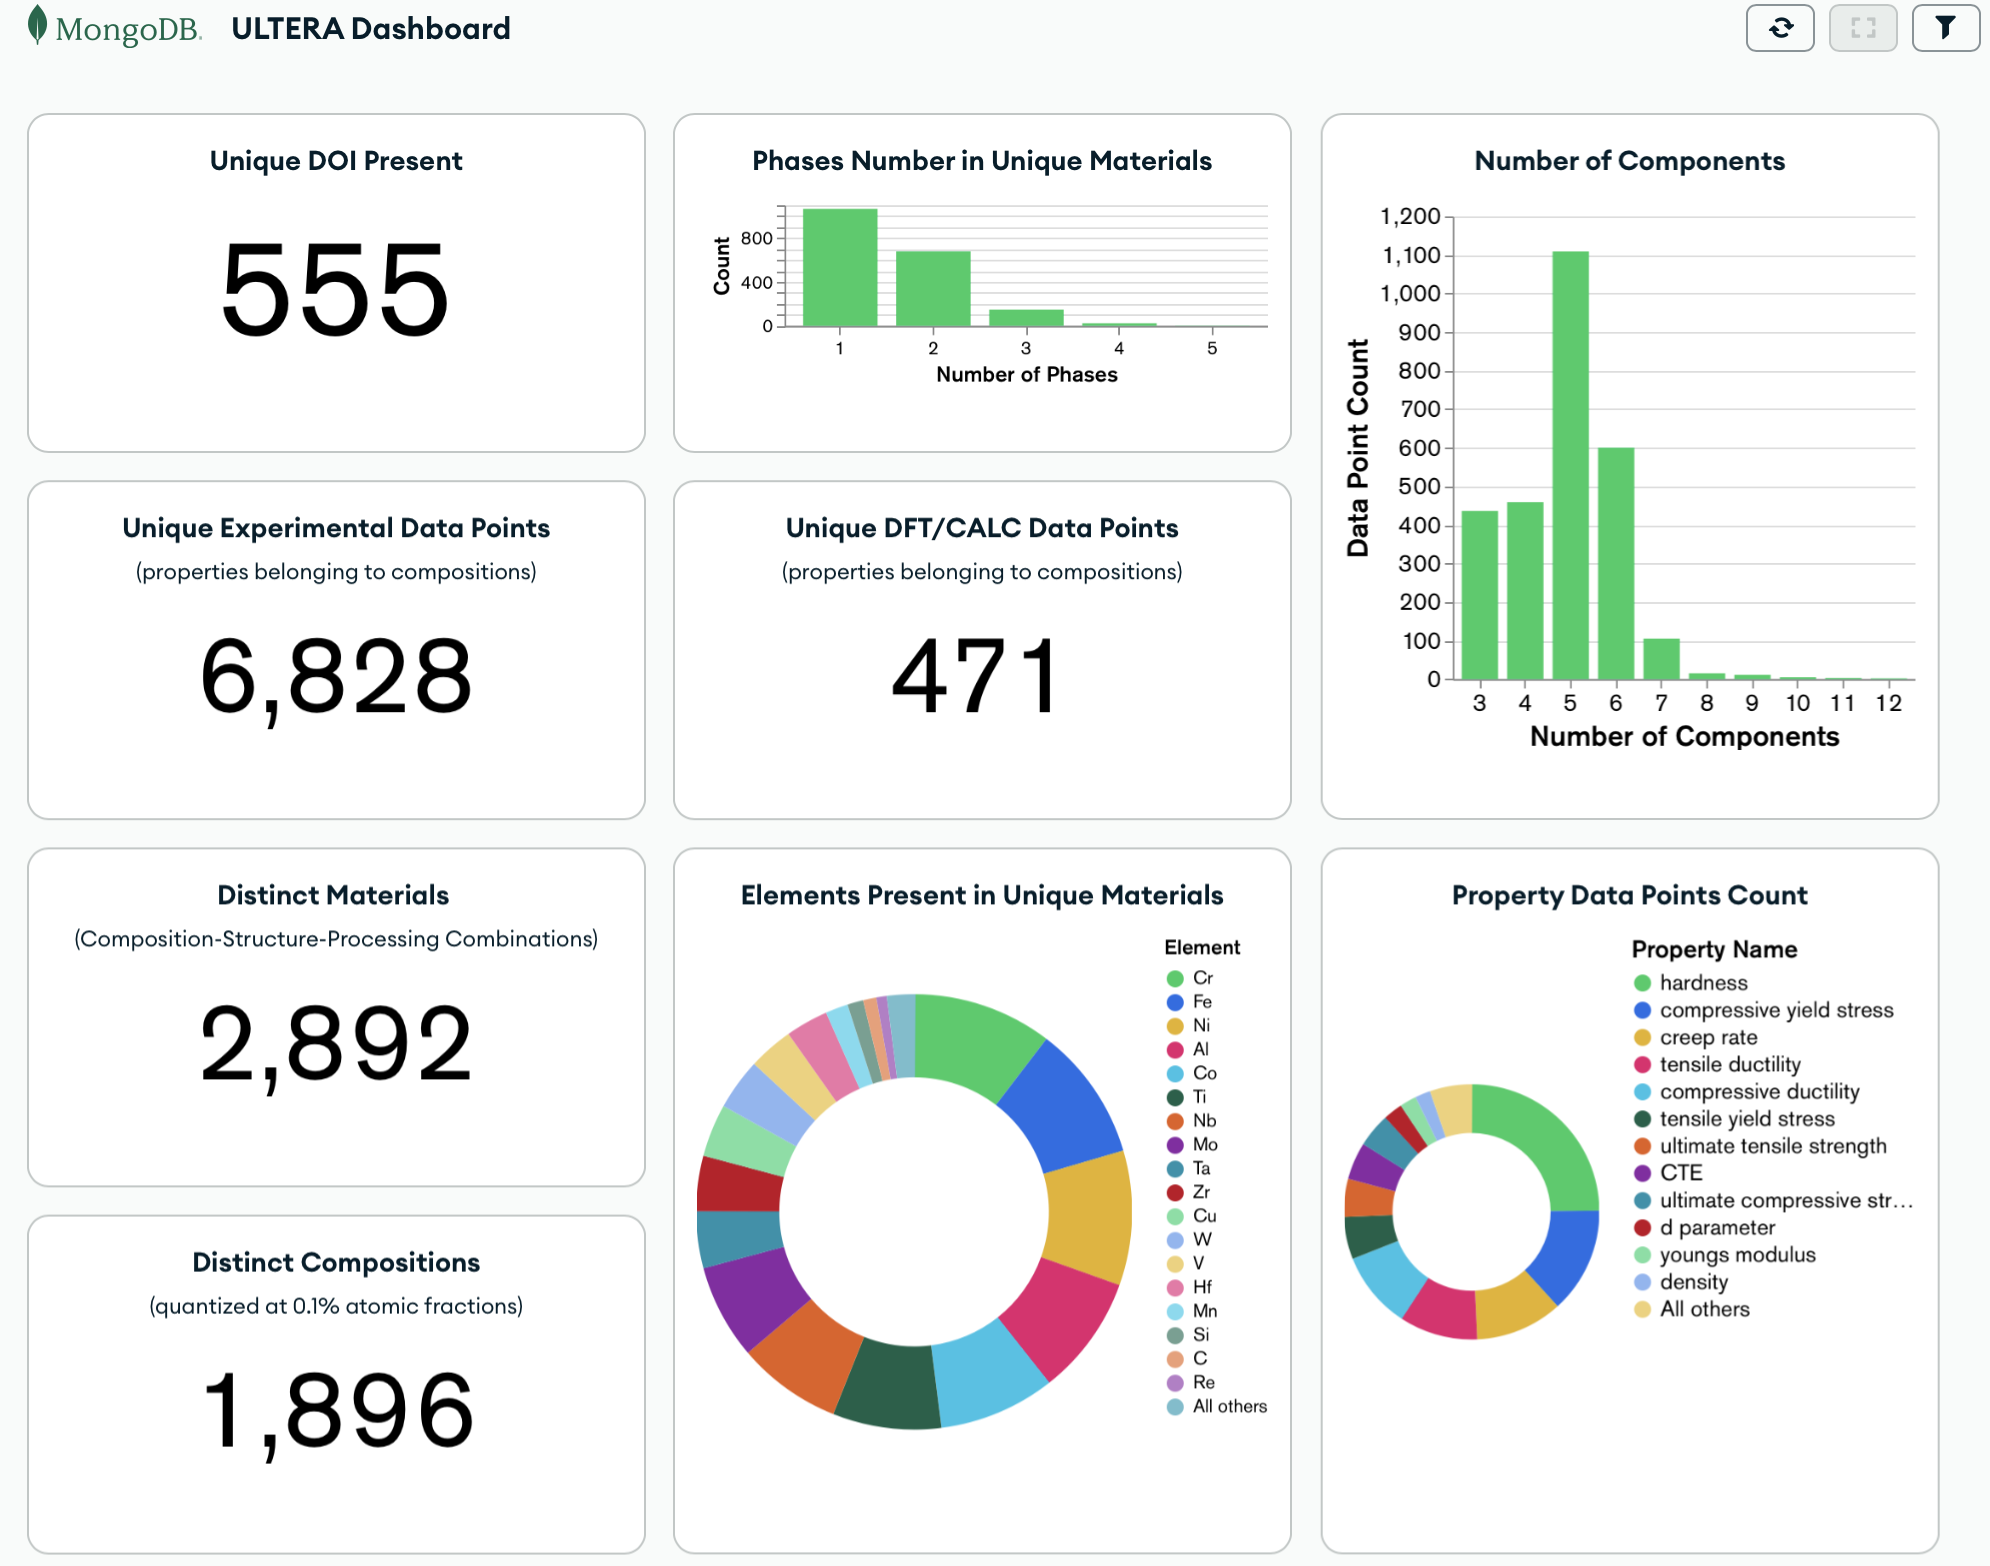
\includegraphics[width=0.95\textwidth]{ultera/ULTERA_Dashboard.png}
    \caption{The main section of \texttt{ULTERA} Database dashboard at \href{https://ultera.org}{ultera.org}; presents statistics as of \statisticstime. All included figures are live and automatically recalculated every 1h. They are interactive allowing users to, e.g., select, highlight, or export the plot data in machine-readable format.}
    \label{ultera:fig:dashboard}
\end{figure}

As depicted in the bottom part of Figure~\ref{ultera:fig:dashboard}, the dataset covers a diverse set of (a) properties and (b) chemical elements. The property set spans 12 with at least 130 datapoints present, with 10 coming from experiments and 2 from computation, with the most common being hardness ($24.6\%$), tensile or compressive ductility ($19.7\%$), tensile or compressive yield stress ($18.9\%$), creep rate ($11.3\%$), and compressive or tensile ultimate strength ($9.1\%$).

The chemical space coverage spans 37 elements, with no bias towards a small subset of them, that most commonly co-occur in 5-component systems, as shown in Figure~\ref{ultera:fig:dashboard}. Out of the chemical elements, 20 are present in at least 80 unique alloys, as listed in Figure~\ref{ultera:fig:chemistries}, making them suitable for ML studies.

\begin{figure}[H]
    \centering
    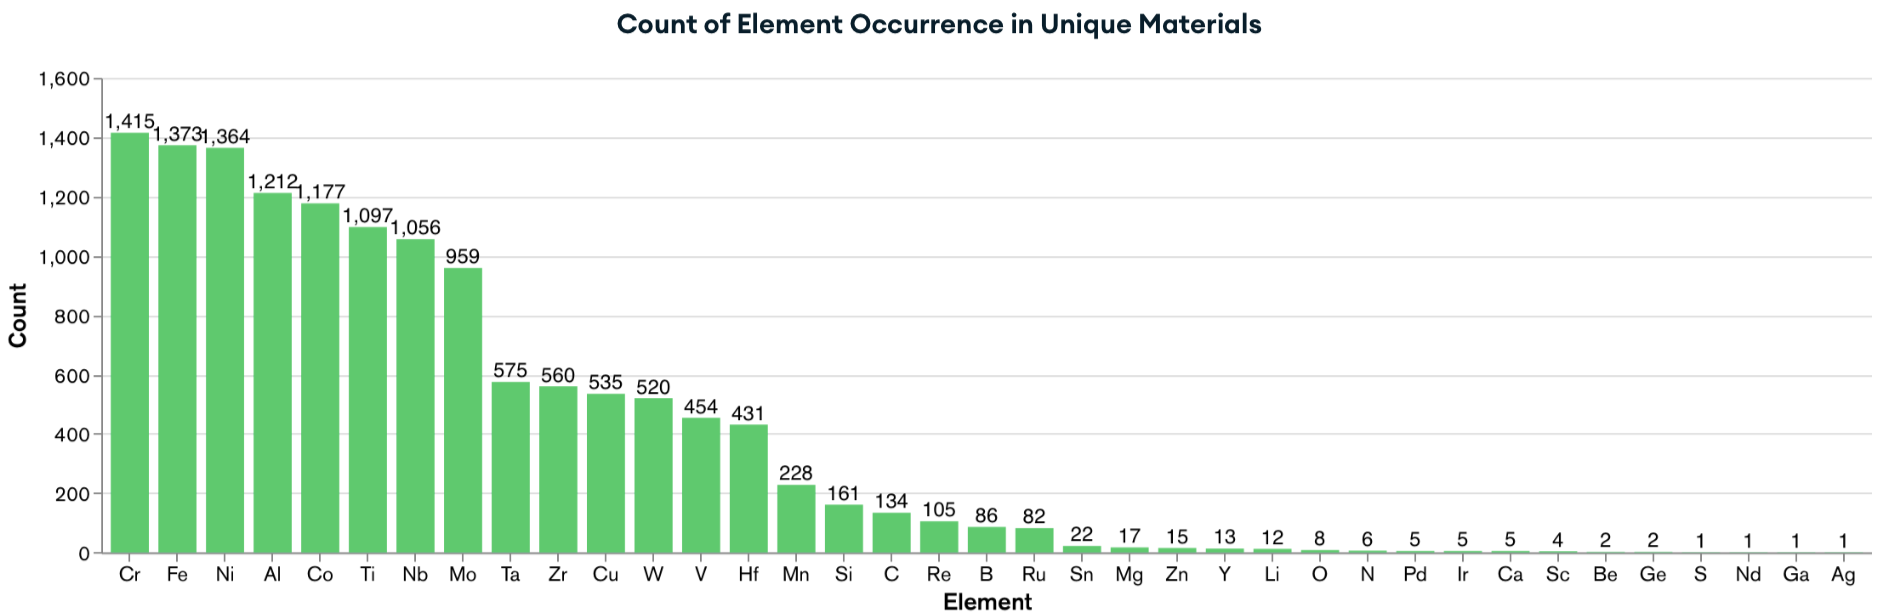
\includegraphics[width=0.95\textwidth]{ultera/ultera_Chemistries.png}
    \caption{Chemical elements in the unique materials collection of the ULTERA Database as of \statisticstime. Please note that the same formula-processing-structure triplet can often be reported by many groups and is counted here as 1 point.}
    \label{ultera:fig:chemistries}
\end{figure}

For each experimental datapoint, the Crossref (\href{https://www.crossref.org}{crossref.org}) service is automatically queried based on the associated DOI (once per unique DOI) to retrieve a set of metadata associated with the study. This allows ULTERA to also be analyzed in terms of time-distribution of the experimental data which can reveal trends in the community regarding its research output, as shown in Figure~\ref{ultera:fig:publicationyears}, or to analyze trends in the explored alloys chemical spaces over the years. The significance of the latter will likely grow in the future, as it can prevent implicit biases into exploration of what "should work", which can limit innovation and design space exploration.

\begin{figure}[H]
    \centering
    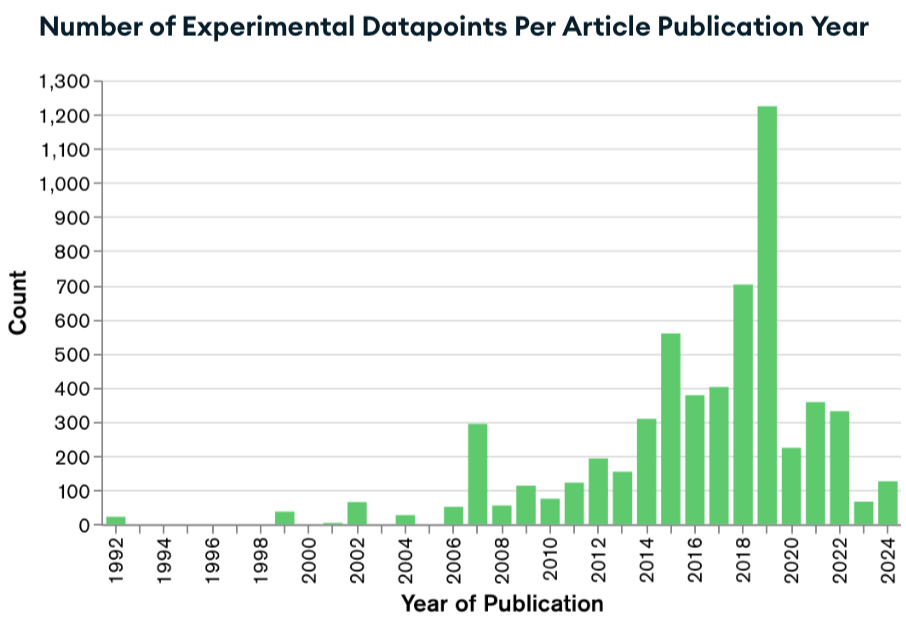
\includegraphics[width=0.7\textwidth]{ultera/ultera_PublicationYear.png}
    \caption{Number of experimental datapoints collected in ULTERA as of \statisticstime vs the year they were published, showing rapid growth. The lower numbers in the last 5 years reported can be attributed to significant portion of the data coming from compilations delayed by 1-3 years and height of COVID pandemic in 2020 delaying experiments.}
    \label{ultera:fig:publicationyears}
\end{figure}

Lastly, it is critically beneficial that every datapoint inserted into the ULTERA's data ecosystem is automatically extended through a number of data homogenization tools, machine learning models, and empirical models, described in later sections, which become immediately available to both modeling researchers (through an API) and data end-users. While much less accurate compared to proper investigations, their complete (or near-complete) coverage is a unique asset, as it puts all materials in the same context, visualizing trends over the entire database, as shown in Figure~\ref{ultera:fig:insights}.

\begin{figure}[H]
    \centering
    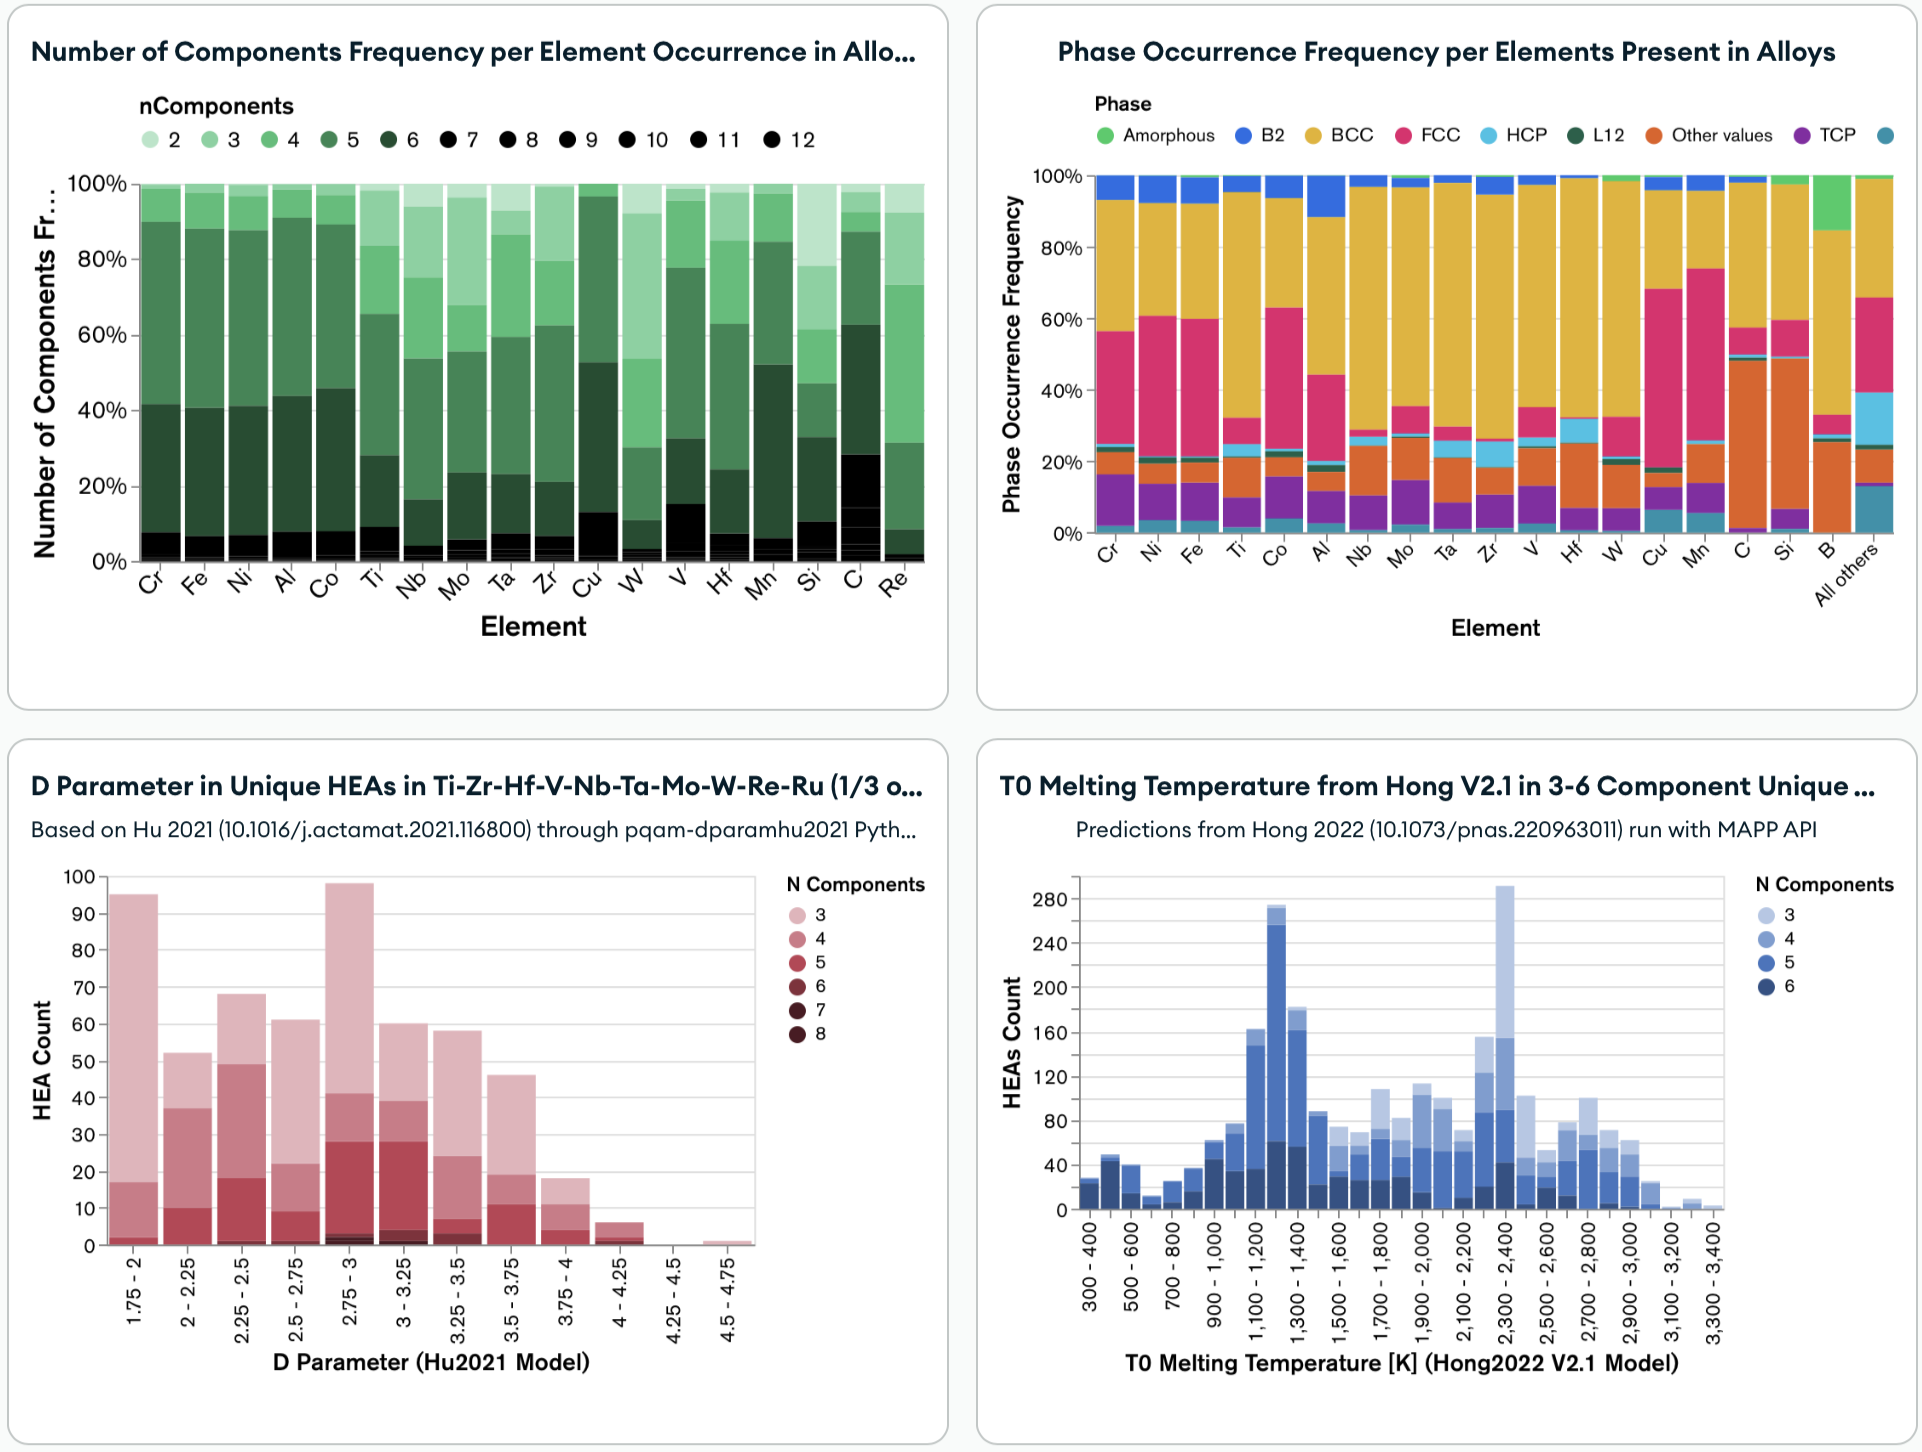
\includegraphics[width=0.95\textwidth]{ultera/ULTERA_Insights.png}
    \caption{A large compiled dataset allows insights into prior expert knowledge driving the discovery and possible biases models generating new alloys will be subject to. The automated data infrastructure, described in Section \ref{ultera:sec:infrastructure}, enables efficient deployment of many tools, such as community models described in Subsection \ref{ultera:ssec:communitymodels}.}
    \label{ultera:fig:insights}
\end{figure}


\section{Alloy Discovery Infrastructure} \label{ultera:sec:infrastructure}

The ULTERA Alloy Discovery Infrastructure, first published conceptually in 2021 \cite{Debnath2021GenerativeAlloys}, is based on a multi-loop paradigm, where the \emph{literature} loop, which collects and extracts as much past knowledge as possible, feeds into the \emph{inverse design} loop, which proposes new alloys based on machine learning (ML) and articifical intelligence (AI) techniques, which are lastly verified experimentally and computationally through \emph{validation loop}, while forward models in the \emph{predictive loop} are developed to fill in the gaps in the knowledge, as depicted in Figure~\ref{ultera:fig:dataloops}. All of the loops are handled by largely independent sub-teams with specific expertise, while the communication of the data between them is facilitated through the ULTERA Database, from which novel alloys are "harvested" after verification.

\begin{figure}[H]
    \centering
    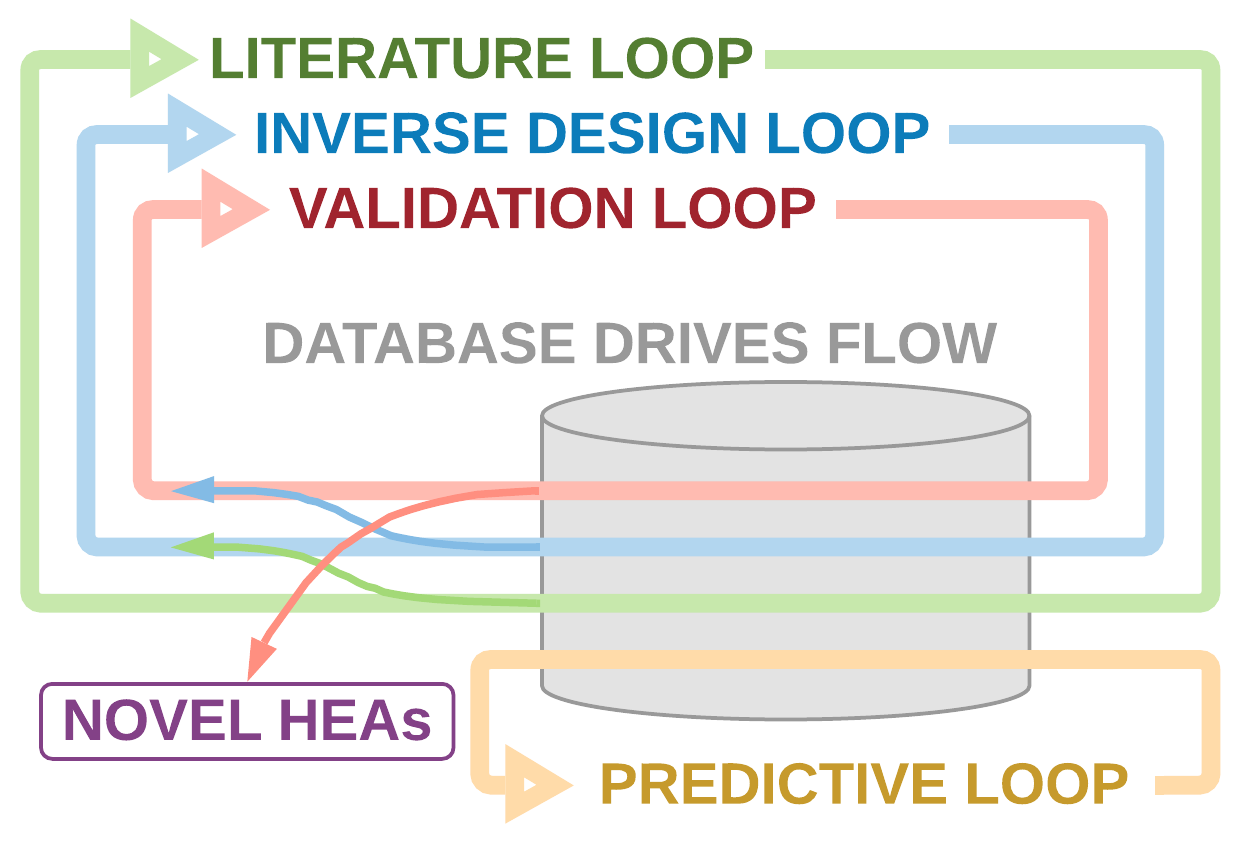
\includegraphics[width=0.5\textwidth]{ultera/PersepctivePaper_DataFlow_V2.png}
    \caption{Four \emph{data loops} associated with different parts of the alloy discovery efforts and the database driving information flow between them to arrive at novel high entropy alloys.}
    \label{ultera:fig:dataloops}
\end{figure}

The flow presented in Figure~\ref{ultera:fig:dataloops} can be expanded in terms of the most critical tasks in each loop to arrive at the more complete picture presented in Figure~\ref{ultera:fig:dataschematic}. As shown, the data infrastructure component of the ULTERA ecosystem focuses on efficiently combining multiple internal and external data sources and then reorganizes it, as explored in detail later in Section~\ref{ultera:sec:pipeline}. In the process, two individual "databases" are created from the end-user perspective. 

The first one, called \texttt{CURATED} collection, is a "database" centered around individual property datapoints, which allows quick investigation in a format akin to literature publication tables and can be used to efficiently query for property data following certain criteria, such as property name being "tensile yield strength", containing chemical element "Mo", and being measured at temperatures between $270K$ and $300K$, to establish datasets for single-property machine learning models.

The second one, called \texttt{AGGREGATED} collection, is a "database" centered around unique materials (composition-structure-processing triplets), which allow efficient merging of properties from multiple studies and models to construct as complete picture as possible around the defined alloys. It serves as the query point for (1) selection of next experiments and other valudations, (2) identification of what critical data may be missing and should be looked for in the literature, and (3) more elaborate machine learning efforts that leverage correlations between properties to improve individual performance.

\begin{figure}[H]
    \centering
    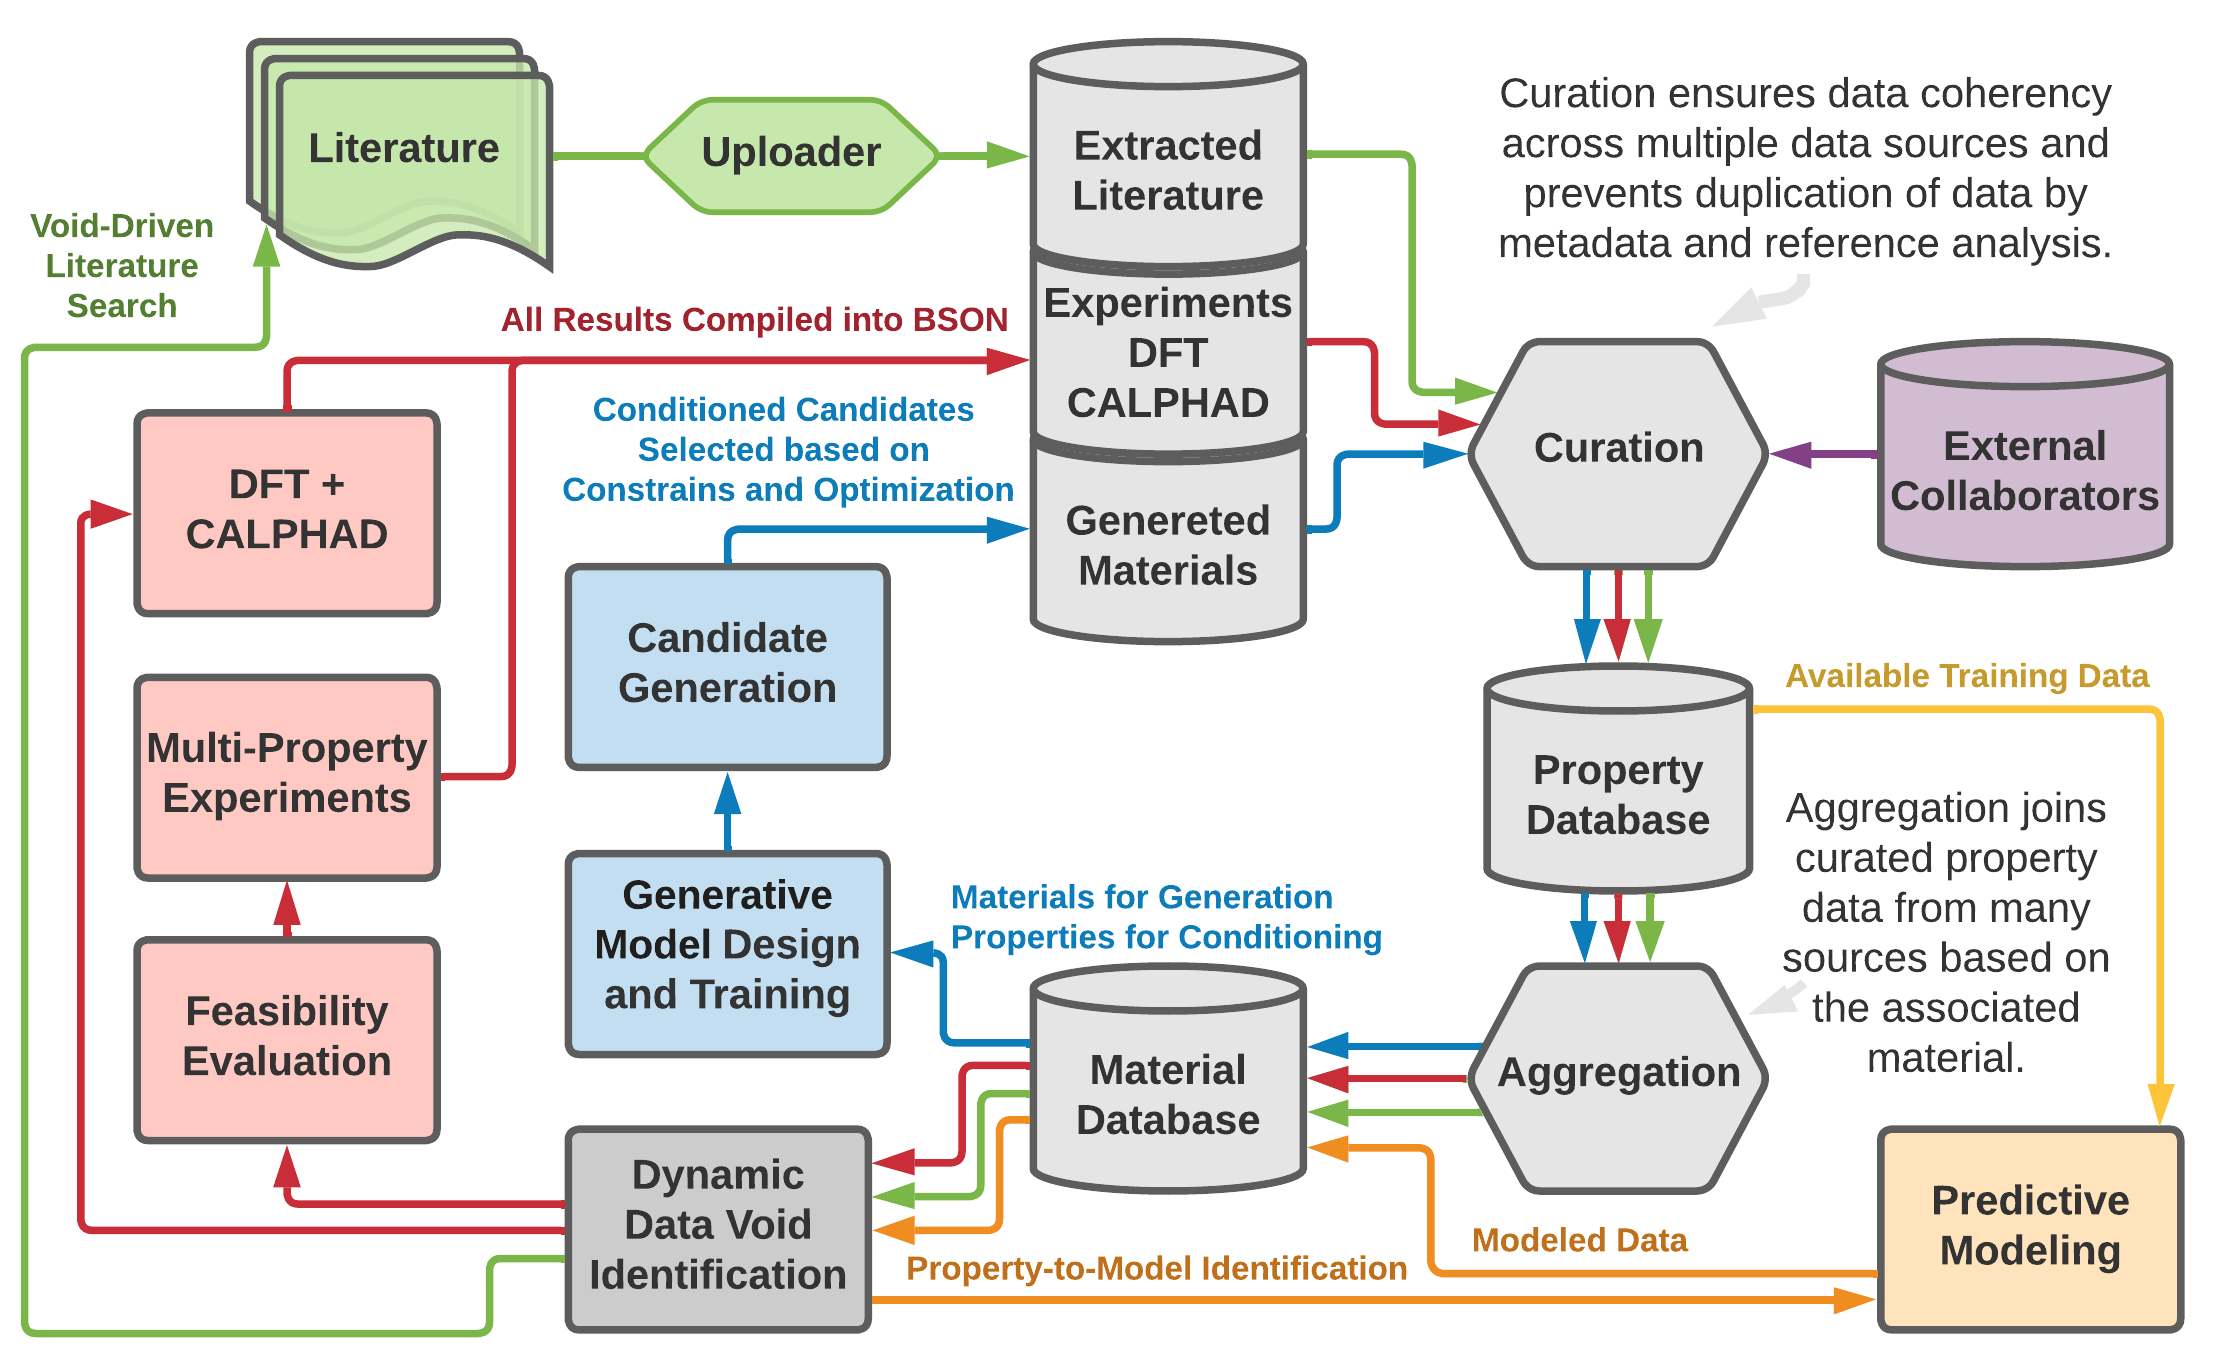
\includegraphics[width=0.9\textwidth]{ultera/PersepctivePaper_Ecosystem_V6.png}
    \caption{Big picture schematic of the ULTERA Data Infrastructure composed of the literature loop (green) collecting available external knowledge from many sources, the predictive loop (orange) filling in the gaps in current state of knowledge with modeling data, the generative loop (blue) proposing new candidate alloys to evaluate, validation loop (red) performing calculations and experiments to validate candidates. In the process databases are created, containing \texttt{CURATED} subset of materials property data, then \texttt{AGGREGATED} around unique materials for multi-property learning. The underlying infrastructure includes many more data collections hidden from users to enable efficient pipelines.}
    \label{ultera:fig:dataschematic}
\end{figure}

Together, all of the loops in ULTERA Infrastructure form a cyclic ecosystem with majority of the steps being automated (except for experiments and literature parsings), thus creating nearly self-driving driving infrastructure capable of automatically extending itself.


\section{Data Pipeline} \label{ultera:sec:pipeline}

Between the data being inserted into the ULTERA ecosystem and presented to the end-user, several key operations are performed, as schematically depicted in Figure~\ref{ultera:fig:datapipeline}. First, the raw data point is passed through an \texttt{uploader} script, which attempts to interpret its the material definition and associated property data into a standardized structure while assigning metadata related to its provenance. At the same time, it performs a number of rule-based and pattern-based checks, related to the data schema, which verify data \emph{can} be valid based on, e.g., presence of required fields and correct data types.


\begin{figure}[H]
    \centering
    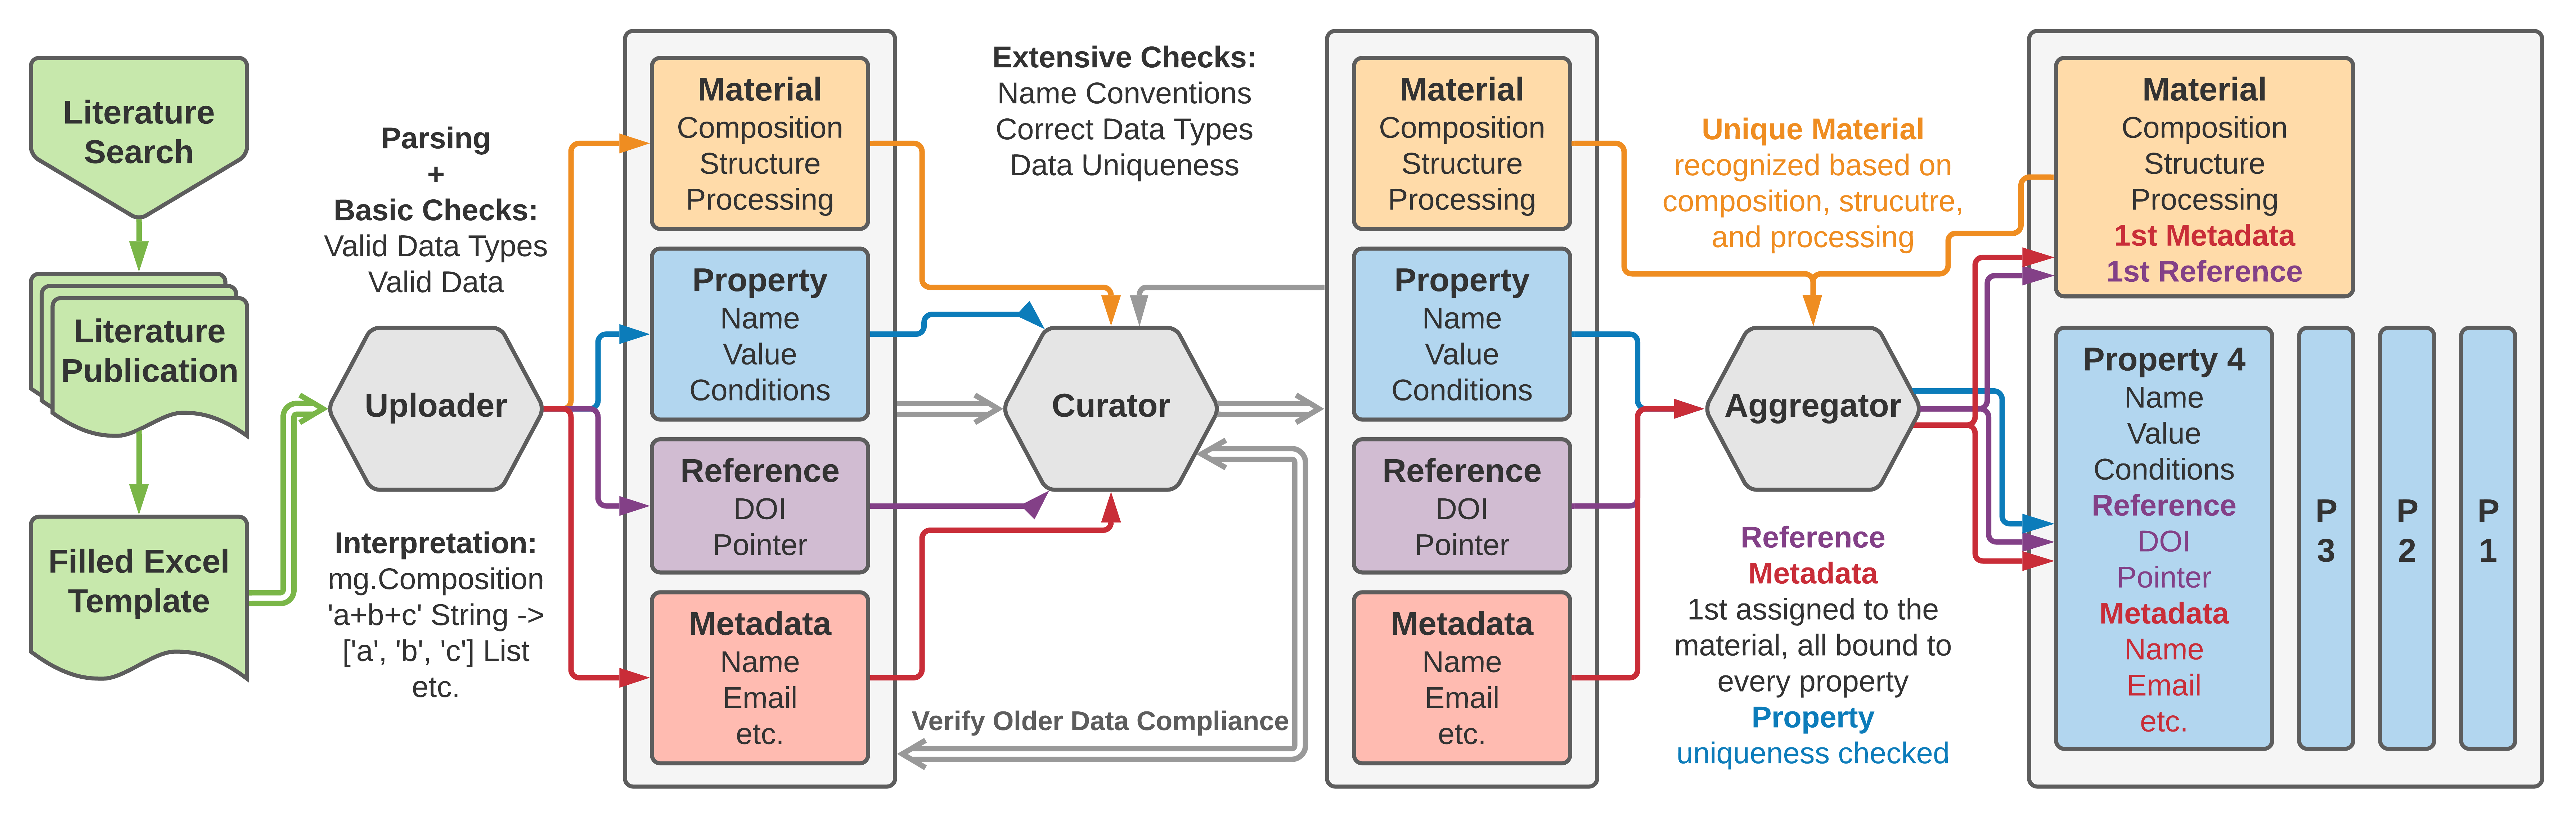
\includegraphics[width=0.95\textwidth]{ultera/ULTERA Data Detail.png}
    \caption{Schematic of the forward pipeline applied to data ingested into the system. For conciseness, intermediate steps of curation process and associated intermediate datasets are not depicted. Critically, a number of data points can converge at each step, so backward trace would be highly branched.}
    \label{ultera:fig:datapipeline}
\end{figure}

Next, a set of curating scripts perform a set of checks both forward (as data gets uploaded) and backwards (on past uploaded data) to ensure that all of it is compliant to the current specification. While there is some overlap with the uploading step, the curation is much more extensive and puts data points in the context of the entire database to enable, e.g., ensuring the uniqueness of the data present. This approach enables ULTERA to avoid both obvious duplicates (accidental second upload) and hidden duplicates (one study reporting data from another without acknowledging the source). It also features homogenization mechnisms, such as converting names based on conventions, e.g., mapping "tensile ultimate strength" and "UTS" to "ultimate tensile strength", while providing reports of compliance to the data administrator. After the curation step, the data is cast into a schema exemplified with the code below and cast into the \texttt{CURATED} collection.

\begin{minted}[xleftmargin=3\parindent, linenos=true, fontsize=\small]{json}
{
  "_id": {
    "$oid": "638a980130b7ffbd9fa64947"
  },
  "meta": {
    "source": "LIT",
    "name": "Hui Sun",
    "email": "suh960@psu.edu",
    "directFetch": "T",
    "handFetch": "T",
    "comment": 
      "Data originally fetched by Hui, but heavily edited and re-uploaded by Adam",
    "timeStamp": {
      "$date": "2022-12-03T00:27:40.005Z"
    },
    "dataSheetName": "HuiAdam_FractureToughnessHardnessDataUpdate_Jan2022_AdamFix.xlsx",
    "sourcePriority": 2,
    "duplicates": [],
    "dataPointsCount": 1
  },
  "material": {
    "rawFormula": "ZrNbMoHfV",
    "formula": "Hf1 Zr1 Nb1 V1 Mo1",
    "compositionDictionary": {
      "Zr": 0.2,
      "Nb": 0.2,
      "Mo": 0.2,
      "Hf": 0.2,
      "V": 0.2
    },
    "percentileFormula": "Hf20 Zr20 Nb20 V20 Mo20",
    "relationalFormula": "Hf1 Zr1 Nb1 V1 Mo1",
    "compositionVector": 
        [ 0, 0, 0, 0, 0, 0, 0.2, 0.2, 0.2, 0.2, 0, 0, 0.2, 0, 0, 0, 0, 0, 0, 0
    ],
    "anonymizedFormula": "ABCDE",
    "reducedFormula": "HfZrNbVMo",
    "system": "Hf-Mo-Nb-V-Zr",
    "elements": [ "Hf", "Mo", "Nb", "V", "Zr" ],
    "nComponents": 5,
    "structure": [
      "BCC",
      "laves"
    ],
    "nPhases": 2,
    "observationTemperature": 298,
    "singleSolidSolution": false,
    "solidSolution": false
  },
  "property": {
    "name": "hardness",
    "value": 5285973000,
    "source": "EXP",
    "temperature": 298
  },
  "reference": {
    "doi": "10.1179/1432891714Z.000000000785",
    "pointer": "P769",
    "doiCount": 1,
    "citation": "Guo, N.N., Luo, L.S., Su, Y.Q. and Guo, J.J. 2014. Microstructure ...",
    "bibentry": " @article{Guo_2014, title={Microstructure and mechanical properties ...",
    "authors": [
      "N. N. Guo",
      "L. S. Luo",
      "Y. Q. Su",
      "J. J. Guo"
    ],
    "dateCreated": {
      "$date": "2014-08-05T00:00:00.000Z"
    },
    "title": "Microstructure and mechanical properties of ZrNbMoHfV high entropy alloy"
  },
  ...
}
\end{minted}

Finally, the aggregation step extracts the material definition from each datapoint present in the \texttt{CURATED} collection and groups them based on their uniqueness, while applying priority rules to establish precedence of original studies over reviews and reviews over larger datasets. During the grouping, most of the auxiliary data (metadata and reference information) are added to a set, while actual data is organized as ordered lists, to arrive at a schema exemplified with the code below and cast into the \texttt{AGGREGATED} collection.

\begin{minted}[xleftmargin=3\parindent, linenos=true, fontsize=\small]{json}
{
  "_id": {
    "$oid": "666956c247f65c310dae9e94"
  },
  "material": {
    "formula": "Zr1 Ti1 Ta1 Nb1 Mo1",
    "compositionDictionary": {
      "Ti": 0.2,
      "Ta": 0.2,
      "Nb": 0.2,
      "Mo": 0.2,
      "Zr": 0.2
    },
    "percentileFormula": "Zr20 Ti20 Ta20 Nb20 Mo20",
    "relationalFormula": "Zr1 Ti1 Ta1 Nb1 Mo1",
    "compositionVector": 
      [ 0, 0, 0, 0, 0, 0.2, 0.2, 0.2, 0.2, 0, 0, 0.2, 0, 0, 0, 0, 0, 0, 0, 0
    ],
    "anonymizedFormula": "ABCDE",
    "reducedFormula": "ZrTaTiNbMo",
    "system": "Mo-Nb-Ta-Ti-Zr",
    "elements": [
      "Mo",
      "Nb",
      "Ta",
      "Ti",
      "Zr"
    ],
    "nComponents": 5,
    "structure": [
      "BCC",
      "BCC"
    ],
    "nPhases": 2,
    "processes": [
      "AC"
    ],
    "nProcessSteps": 1,
    "singleSolidSolution": false,
    "solidSolution": true,
    "rawFormulas": [
      "TiTaNbMoZr",
      "MoNbTaTiZr"
    ],
    "observationTemperatures": [ 1273, 800, 323, 298, 298, 298 ]
  },
  "properties": [
    {
      "name": "CTE",
      "value": 0.0000075,
      "source": "EXP",
      "temperature": 323,
      "unitName": "K^-1",
      "sourcePriority": 3,
      "meta": {
        "source": "LIT",
        "name": "Adam Krajewski",
        "email": "ak@psu.edu",
        "directFetch": "T",
        "handFetch": "T",
        "comment": "HEA CTE search effort",
        "timeStamp": {
          "$date": "2023-07-08T00:02:37.218Z"
        },
        "dataSheetName": "ULTERA-contribute-amkrajewski/ThermalExpansionSearch_Oct22.xlsx",
        "sourcePriority": 2,
        "duplicates": [],
        "dataPointsCount": 1
      },
      "reference": {
        "doi": "10.1016/j.jallcom.2021.162154",
        "pointer": "F6",
        "doiCount": 3
      }
    },
    {
      "name": "ultimate compressive strength",
      "value": 1450000000,
      "source": "EXP",
      "temperature": 298,
      "sourcePriority": 3,
      "meta": {
        "source": "LIT",
        "parentDatabase": "MPEA",
        "name": "Adam Krajewski",
        "email": "ak@psu.edu",
        "directFetch": "F",
        "handFetch": "F",
        "comment": "Alloys from Citrine / UCSB HEA Database as of August 2021",
        "timeStamp": {
          "$date": "2022-12-02T23:53:44.918Z"
        },
        "dataSheetName": "ULTERA_MEPA_combineddata.xlsx",
        "sourcePriority": 2,
        "duplicates": [],
        "dataPointsCount": 1
      },
      "reference": {
        "doi": "10.1016/j.scriptamat.2016.10.028",
        "doiCount": 4
      }
    },
    ...
  ],
  "parents": [
    {
      "$oid": "64a8a7ab9e7f829350cce73e"
    },
    {
      "$oid": "64a8a7ab9e7f829350cce73f"
    },
    ...
  ],
  "uploaders": [
    "Adam Krajewski"
  ],
  "metaSet": [
    {
      "source": "LIT",
      "name": "Adam Krajewski",
      "email": "ak@psu.edu",
      "directFetch": "T",
      "handFetch": "T",
      "comment": "HEA CTE search effort",
      "timeStamp": {
        "$date": "2023-07-08T00:02:37.218Z"
      },
      "dataSheetName": 
        "ULTERA-contribute-amkrajewski/ThermalExpansionSearch_Oct22.xlsx",
      "sourcePriority": 2,
      "duplicates": [],
      "dataPointsCount": 1
    },
    ...
  ],
  "referenceSet": [
    {
      "doi": "10.1016/j.msec.2016.12.057",
      "doiCount": 1
    },
    {
      "doi": "10.1016/j.scriptamat.2016.10.028",
      "doiCount": 4
    },
    {
      "doi": "10.1016/j.jallcom.2021.162154",
      "pointer": "F6",
      "doiCount": 3
    }
  ],
}
\end{minted}


In addition to the \texttt{CURATED} and \texttt{AGGREGATED} collections depicted in Figure~\ref{ultera:fig:dataschematic}, there are several other that are hidden from the end-user but perform critical functions as intermediate stages, deployment targets, and provenance metadata sources. These are:

\begin{itemize}
    \item Many (20+) individual user-specific or source-specific data collections with fine-grained permissions assigned based on current stewardship distribution. 


    \item \texttt{ALL} - combines (nearly) all source collections into one for further processing using MongoDB aggregation pipelines, after trimming fields that were empty (due to, e.g., single whitespace in spreadsheet) and removing test data entries marked with comments like \texttt{'test'}.


    \item \texttt{STRUCTURAL} - which groups the \texttt{CURATED} collection around unique materials \emph{except for processing history, comments, and observation temperature} to act as a deployment target for models taking into account alloy composition and structure.


    \item \texttt{COMPOSITIONAL} - which groups the \texttt{CURATED} collection around unique materials \emph{except for structure-related fields, processing history, comments, and observation temperature} to act as a deployment target for models taking into account only the alloy composition.


    \item \texttt{DOI} - used to store references based on the DOIs and link back to the \texttt{CURATED} collection. The reference fetching is performed only when new DOI is inserted, but linking is refreshed every time \texttt{CURATED} data changes.

    \item \texttt{CURATED\_Jul2023} and other versioned-backup collections - used to produce results presented in scientific publications.
\end{itemize}

%To better visualize the 

%\begin{figure}[H]
%    \centering
%    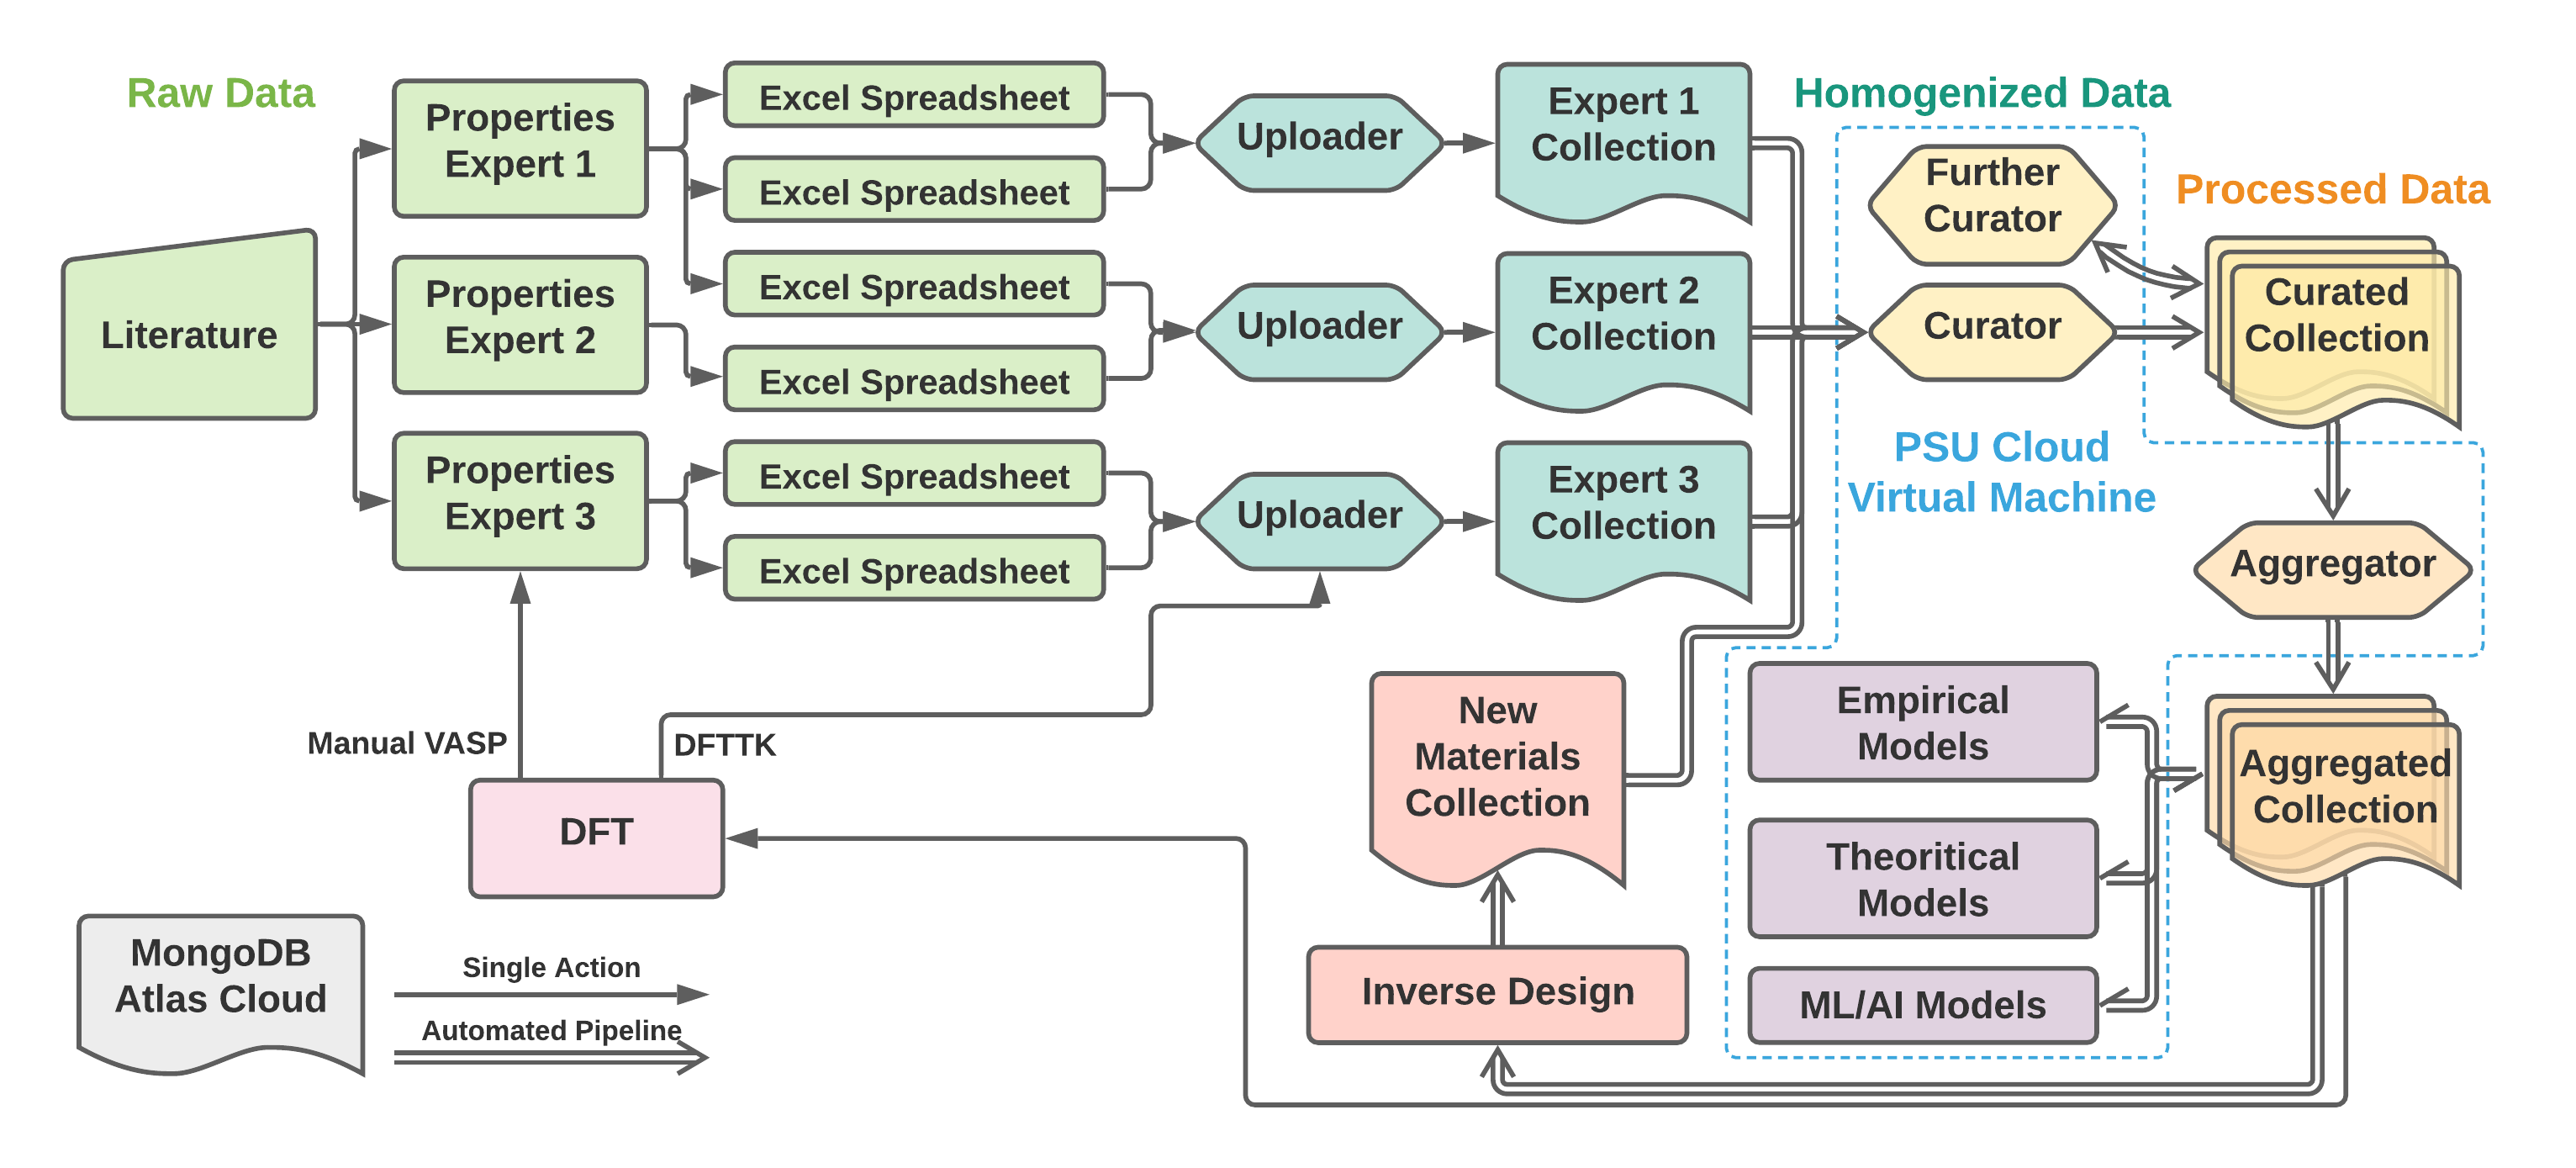
\includegraphics[width=0.95\textwidth]{ultera/ULTERA_Data_Cycle_v2.png}
%    \caption{Schematic of the computational (non-experimental) data flow from perspective closer to the underlying pipelines, with double lines marking fully automated steps happening on the cloud. For conciseness, intermediate steps, like reorientation of data around unique compositional or structural datasets for efficient model deployment are not depicted.}
%    \label{ultera:fig:datacycles}
%\end{figure}

\section{Community Contributions} \label{ultera:sec:contributions}

While ULTERA is internally organized based on a cloud non-relational database with elaborate data processing, explored in Sections \ref{ultera:sec:infrastructure} and \ref{ultera:sec:pipeline}, the majority of data ingested into the system has to pass through researchers not familiar with the ecosystem specifics or programming in general. Thus, a contribution template, shown in Figure~\ref{ultera:fig:contributiontemplate}, has been developed to contain \emph{unprocessed} source data mapping fields shown in Figure~\ref{ultera:fig:material}, needed to construct ULTERA entries.

\begin{figure}[H]
    \centering
    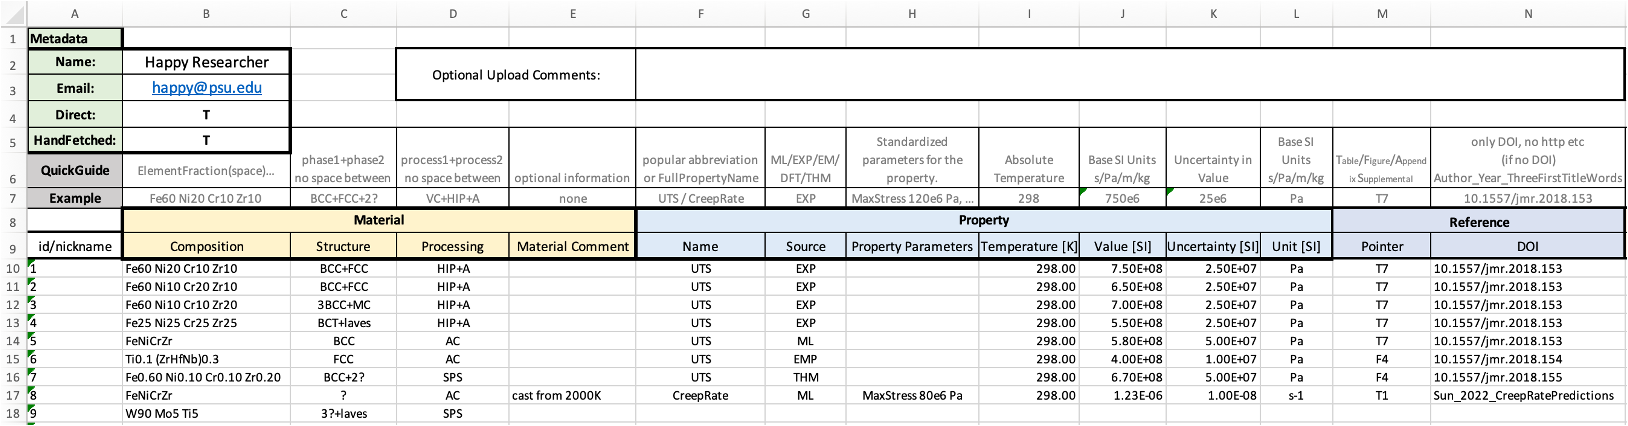
\includegraphics[width=0.97\textwidth]{ultera/ULTERA_Contribute.png}
    \caption{Header and example data rows of a formatted Excel spreadsheet template used to streamline and increase accessibility to the contribution system for non-technical members of the community. An automated system processes them on the cloud into git-tracked plain-text CSV records then passed to uploading system.}
    \label{ultera:fig:contributiontemplate}
\end{figure}

Such spreadsheet templates can be either (a) stored locally and passed manually by users who want to make a small singular contribution, e.g., to accompany a publication, or (b) stored in a \texttt{git} repository on GitHub, which can be linked and automatically ingested into ULTERA based on the internal meta-repository. To simplify the latter, an origin repository has been made available at \href{http://contribute.ultera.org/}{contribute.ultera.org} for forking.

Furthermore, the provided template repository also includes several automations described in its \texttt{README.md}, which are built around GitHub Actions and enable functionalities, such as git-tracking of the Excel's \texttt{XLSX} spreadsheet contents by casting it into plain-text \texttt{CSV} on every push to a branch. In the future when ULTERA will be made fully open, data quality analysis methods, described in Chapter \ref{chap:pyqalloy}, will also be included at this step.


\section{Automatic Modeling} \label{ultera:sec:automodel}

\subsection{Multi-Structure Linear Combinations} \label{ultera:ssec:autolc}



Calculating a linear combination (LC) of "elemental" (or otherwise component) properties is most straightforward approach to estimating property values, especially in cases where phase stability differences play a secondary role, as it presents near-zero computational expense while requiring only readily-available data that has been likely tabulated in some computer-readable format. In most studies, these elemental values are assumed to have one-to-one correspondence with the chemical element. However, while this may hold true for, e.g., price or atomic weight, many elements will behave very differently when in different crystal structures (e.g., Fe in BCC vs FCC).

Thus, in ULTERA, whenever possible, LCs for each alloy are calculated on structure-specific data coming from experiments or multi-lattice ab-initio calculations \cite{Chong2021CorrelationAlloys} stored in a dedicated \texttt{ELEMENTAL} database of ULTERA, to establish different LC values under BCC, FCC, and HCP assumptions, as shown in Figure~\ref{ultera:fig:autolc}. During LC calcualtions, some element-structure pairs are unavoidably missing (e.g. BCC Cu \cite{Chong2021CorrelationAlloys}) but in such cases the missing data with most similar one while tracking the level of it under \texttt{replacementLevel} field. 

\begin{figure}[H]
    \centering
    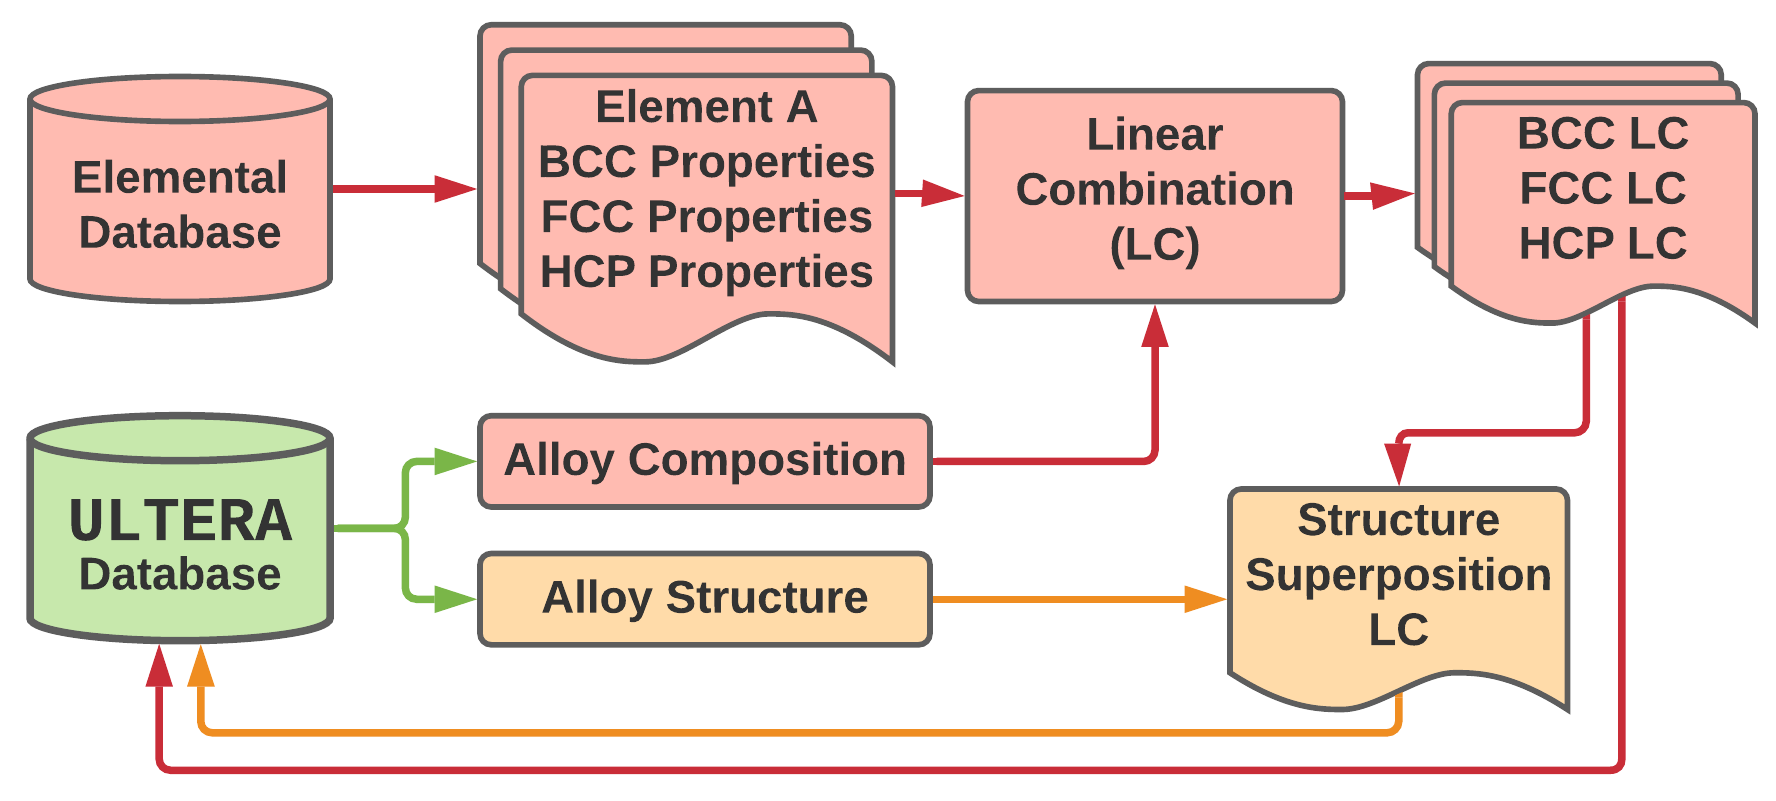
\includegraphics[width=0.6\textwidth]{ultera/ULTERA_ElementalDatabase_LC_V1.png}
    \caption{Simplified schematic of automatic linear combination modeling of properties. For every chemical composition, a linear combination of elemental properties is calculated for BCC, FCC, and HCP structures, based on best-matched elemental polymorph data coming from experiments and DFT-based pure element calculations. If applicable structure set (e.g., FCC+FCC+HCP) has been reported for a given input datapoint, an average of the respective linear combinations is reported as structure-informed LC.}
    \label{ultera:fig:autolc}
\end{figure}

If a datapoint has a structure (either single- or multi-phase) reported for it, then an additional LC is calculated to reflect an average of the structure-specific LCs weighted by the number of given phases being reported, or when possible, by the exact phase fractions coming from CALPHAD equilibrium or solidification (e.g., Scheil \cite{Bocklund2020ExperimentalMaterials}) calculations run through \texttt{pycalphad} \cite{Otis2017Pycalphad:Python}. All LCs are then collectively reported under the \texttt{structuralProperties}, arriving at a schema exemplified with the code below.

\begin{minted}[xleftmargin=3\parindent, linenos=true, fontsize=\small]{json}
{
  "_id": {
    "$oid": "638a980130b7ffbd9fa64947"
  },
  ...
  "structuralProperties": {
    "LC_BCC": {
      "replacementLevel": 0.4,
      "SQusf": 0.68966,
      "G111C": 63.489999999999995,
      "DFTC12": 117.67000000000002,
      "DFTGvb": 18.1292,
      "NfUnfill": 0,
      "Heat_Sublimation": 623414.4,
      "Ion_Pot_2": 14.328000000000001,
      "Surf": 2.2020000000000004,
      ...
    },
    "LC_FCC": {
      "replacementLevel": 0.6,
      "SQusf": 0.6138399999999999,
      "G111C": 57.824,
      "DFTC12": 123.278,
      "DFTGvb": 21.0182,
      "NfUnfill": 0,
      "Heat_Sublimation": 623414.4,
      "Ion_Pot_2": 14.328000000000001,
      "Surf": 2.116,
      ...
    },
    "LC_HCP": {
      "replacementLevel": 0.6,
      "SQusf": 0.68966,
      "G111C": 63.489999999999995,
      "DFTC12": 117.67000000000002,
      "DFTGvb": 18.1292,
      "NfUnfill": 0,
      "Heat_Sublimation": 623414.4,
      "Ion_Pot_2": 14.328000000000001,
      "Surf": 2.2020000000000004,
      ...
    }
  }
}
\end{minted}



\subsection{Community Model Deployment} \label{ultera:ssec:communitymodels}

As mentioned in Section \ref{ultera:sec:intro}, the ULTERA Infrastructure automatically deploys several literature models onto all applicable datapoints. These include melting temperature ($T_0$) predictions by \citet{Hong2022MeltingMaterials}, intrinsic ductility prediction by \citet{Hu2021ScreeningAlloys}, root mean square atomic displacement in BCC HEA by \citet{Tandoc2023MiningAlloys}, or formation energy by \citet{Krajewski2022ExtensibleNetworks}. The utilized pipeline has been designed to be relatively straightforward and can be defined to deploy a model on both full description of a material and partial one (e.g., in \texttt{COMPOSITIONAL} collection) to optimize number of model evaluations.

\begin{minted}[xleftmargin=3\parindent, linenos=true, fontsize=\small]{json}
{
  "_id": {
    "$oid": "638a980130b7ffbd9fa64947"
  },
  ...
  "compositionalProperties": {
    "TM[K]_HongV2_1": {
      "mean": 2322,
      "standard error": 294
    },
    "rmsad_Tandoc2023": 0.18933359511558134,
    "dparam_Hu2021": 2.884705648963465,
    "gfse_Hu2021": 0.6816671231315389,
    "surf_Hu2021": 1.966409000810224,
    "CH_SIPFENN_NN30": -0.03186363223940135,
    ...
  },
  "structuralProperties": {
    "DPARAM_AllData": 2.6416306495666504,
    "DPARAM_Validated": 2.774862051010132,
    "EF_SIPFENN_NN30_BCC": -0.009082297794520855,
    "EF_SIPFENN_NN30_FCC": -0.0027202172204852104,
    "EF_SIPFENN_NN30_HCP": 0.03427823260426521,
    ...
  }
}
\end{minted}


\subsection{Automated CALPHAD Modeling} \label{ultera:ssec:autocalphad}

A more robust pipeline has been created to automatically deploy results of CALPHAD \cite{Olson2023GenomicDynamics} based calculations, into the \emph{modeled} \texttt{compositionalProperties} fields of end-user collections, whenever such calculation can be performed given chemical compositions scope of a given thermodynamic database (TDB), such as one created by Shuang Lin and shared through a GitHub repository \cite{LinShuangLin212/refractory-elements-database:ZR}. Lin's TDB was used to generate the example of data structure below, where one can see, that the reported data contains several phase equilibrium calculation results, including metadata, phase fractions under \texttt{phaseDict} (assuming no miscibility gaps, i.e., two BCC phases are counted as one) and \texttt{phaseFullDict}, presented in two formats, as well as \texttt{zpfPositions} which give zero-phase-fraction (ZPF) points critical to interpretation of experimental results \cite{Li2024DesignExperiments} and modeling phase stability with AI approaches \cite{Wu2023EstimatingApproach}.

\begin{minted}[xleftmargin=3\parindent, linenos=true, fontsize=\small]{json}
{
  "_id": {
    "$oid": "638a980130b7ffbd9fa64947"
  },
  ...
  "compositionalProperties": {
    ...
    "calphad_Feb2023": {
      "T": 1473,
      "TDB": "CrHfMoNbTaTiVWZr_9element_Feb2023",
      "calphadStructure": "BCC+C15",
      "phaseDict": {
        "BCC_A2": 0.817,
        "LAVES_C15": 0.183
      },
      "phaseFullDict": {
        "BCC_A2": 0.817,
        "LAVES_C15": 0.183
      },
      "nPhases": 2,
      "phaseDictString": "{'BCC_A2': 0.817, 'LAVES_C15': 0.183}",
      "phaseFullDictString": "{'BCC_A2': 0.817, 'LAVES_C15': 0.183}",
      "zpfPositions": {
        "BCC_A2": {
          "HF": 0.201232305,
          "MO": 0.184393688,
          "NB": 0.244705403,
          "V": 0.15600952,
          "ZR": 0.213659083
        },
        "LAVES_C15": {
          "HF": 0.194433862,
          "MO": 0.269743594,
          "NB": 0.000002969,
          "V": 0.396690129,
          "ZR": 0.139129446
        }
      },
      "BCC_SS": 0,
      "BCC_SSS": 0
    }
  }
}
\end{minted}

In the example shown, the persisted output is not semantically versioned, but rather marked with unique name \texttt{calphad\_Feb2023} corresponding to a well-defined effort of the team. This design choice has been selected based on character of CALPHAD modelling, where iterations of the TDBs are not numerous, while end-users traditionally favor descriptive names, such as \texttt{Shuang\_May2024\_RefractoryBCO}, which are then fixed and backed by a literature publication.


\subsection{MPDD Atomic Configuration Data Fetching} \label{ultera:ssec:mpdd}

Lastly, the ULTERA ecosystem leverages the 4.5 million of atomistic data points discussed in Chapter~\ref{chap:mpdd} to extract some information about the 0K stability of structures in the given alloy's chemical system or its derivatives (including carbides, oxides, and nitrides), as schematically shown in Figure~\ref{ultera:fig:mpdd}. This data be used to augment both (a) generative modeling efforts \cite{Debnath2021GenerativeAlloys}, as convex hull depth will likely be correlated with formation of stable intermetallics, and (b) interpretation of experiments producing compositional maps \cite{Li2024DesignExperiments}, enabling easy identification of observed compounds of alloy's base elements or carbides formed by impurities. 

\begin{figure}[H]
    \centering
    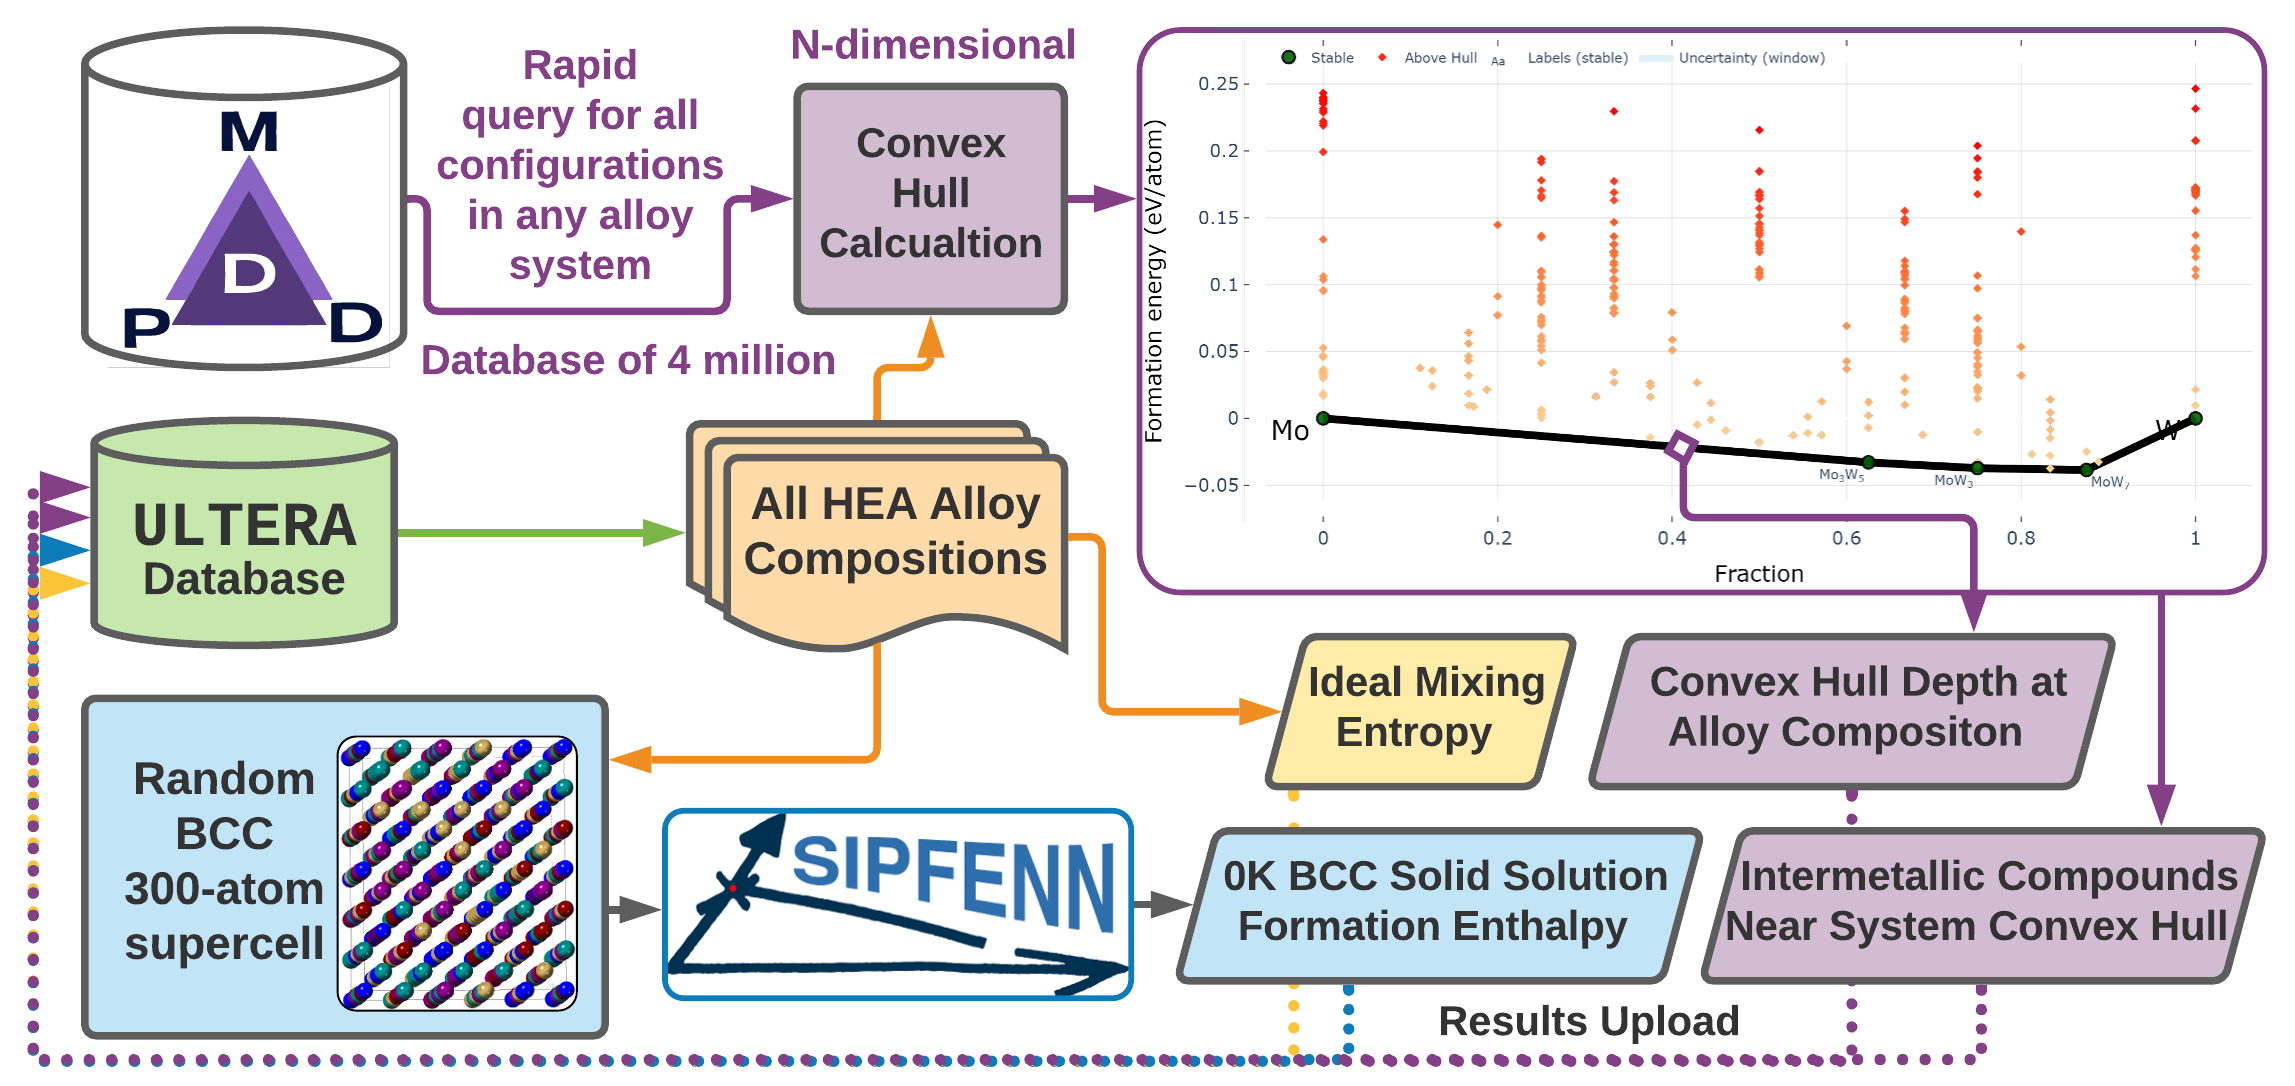
\includegraphics[width=0.8\textwidth]{ultera/ULTERA_BasicThermodynamics_V1.png}
    \caption{Conceptual schematic of how MPDD is directly utilized within ULTERA, going beyond interaction through CALPHAD models, to include basic thermodynamic information. For each composition, a convex hull of compounds present in corresponding chemical system is calculated based on MPDD data and can be used (a) to immediately identify candidates for experimentally observed compounds based on 0K low-energy configurations or (b) convex hull depth can be used as an input to ML model indicating strength of interatomic interactions.}
    \label{ultera:fig:mpdd}
\end{figure}

As shown in an example code below, the acquired data is structured as lists of names constructed from reduced chemical formulas, MPDD unique id, and, if applicable, identifier of the parent source, allowing one to quickly trace back where data came from and fetch additional information. Such schema also allows one to make queries over experimental data based on a specific compound to, for instance, find all literature publication where it may have occured.


\begin{minted}[xleftmargin=3\parindent, linenos=true, fontsize=\small]{json}
{
  "_id": {
    "$oid": "638a980130b7ffbd9fa64947"
  },
  ...
  "compositionalProperties": {
    "carbides_EF_SIPFENN_NN30": [
      0,
      -1.143834464251995,
      -0.2136915735900402,
      -0.10025567188858986,
      -0.1811651661992073,
      -0.4918593931943178,
      ...
    ],
    "carbides_names": [
      "C-60762ac1b003796270f88dcb-cod-1512497",
      "HfC-60da0964462eba27079ee464-aflow:092f750896295d94",
      "Mo4C-60da968d462eba2707adb339-aflow:5c392f4f5bcb399b",
      "MoC-60dbd9c0462eba2707bd846c-aflow:b505b7a2c655c77c",
      "Mo2C-60dc26bd462eba2707c97ba4-aflow:f88a1b395cd63584",
      "NbC-60db3075462eba2707b7bfe9-aflow:949b754227969d87",
      ...
    ],
    "hydrides_EF_SIPFENN_NN30": [
      0,
      -0.4664096124470234,
      -0.30396447144448757,
      -0.44926807284355164,
      -0.26328401267528534,
      -0.25981644354760647,
      ...
    ],
    "hydrides_names": [
      "H2-6075af3cb003796270f4772d-mp-1181189",
      "HfH2-6074fcdbb003796270e70e2d-JVASP-18459",
      "HfH-60752d54b003796270e9d665-OQMD-1234971",
      "HfV2H-60752ef9b003796270ea2c41-OQMD-1287044",
      "MoH2-60752d76b003796270e9e11f-OQMD-1238065",
      "Mo2H-60752d76b003796270e9e11e-OQMD-1238064",
      ...
    ],
    "nitrides_EF_SIPFENN_NN30": [
      0,
      -1.6111129950731993,
      -1.6122573120519519,
      -1.8664569286629558,
      0,
      -0.7383877914398909,
      ...
    ],
    "nitrides_names": [
      "Hf-60752ce4b003796270e9ac2e-OQMD-1214798",
      "HfN-60752ad4b003796270e90b2f-OQMD-1108170",
      "HfVN-60da6fd8462eba2707ab2b4f-aflow:4e079c56a1634e26",
      "HfZrN-60da0169462eba27079d79af-aflow:0144b323e66b8b75",
      "Mo-60da6b40462eba2707aaa2a2-aflow:4b0a71282920e55b",
      "Mo2N-60752d88b003796270e9e5d4-OQMD-1239597",
      ...
    ],
    "oxides_EF_SIPFENN_NN30": [
      0,
      -3.924865636974573,
      -2.6255424302071333,
      0,
      -1.3926446568220854,
      -2.30870558321476,
      ...
    ],
    "oxides_names": [
      "Hf-60752ce4b003796270e9ac2e-OQMD-1214798",
      "HfO2-60dbe621462eba2707bfde2d-aflow:c24b2b7185250bc5",
      "HfO-60dbe7d6462eba2707c0306b-aflow:c41bd454b8f0284b",
      "Mo-60da6b40462eba2707aaa2a2-aflow:4b0a71282920e55b",
      "Mo2O-60752da2b003796270e9eb94-OQMD-1241669",
      "MoO2-6075bbdeb003796270f60c46-mvc-5806",
      ...
    ],
    "stable_EF_SIPFENN_NN30": [
      0,
      -0.16737285256385803,
      -0.14167926087975502,
      -1.0520951068028808,
      -0.046786464750766754,
      -0.07561314664781094,
      ...
    ],
    "stable_names": [
      "Hf-60752ce4b003796270e9ac2e-OQMD-1214798",
      "HfMo2-6074fcb1b003796270e70146-JVASP-14517",
      "Hf2Mo-60752d80b003796270e9e382-OQMD-1238828",
      "HfMo22-60dc048f462eba2707c46fee-aflow:dc1b0e16d62c30a5",
      "HfNb2-60dc12e9462eba2707c6529d-aflow:e6be499b110376f2",
      "HfNb5-60dc29b6462eba2707ca10ea-aflow:fbd6fc861701f121",
      ...
    ],
    ...
  }
}
\end{minted}





\printbibliography[heading=subbibintoc]